%
% STklos + Tk  Documentation
%
%           Author: Erick Gallesio [eg@kaolin.unice.fr]
%    Creation date:  4-Nov-1992 15:37
% Last file update:  5-Jun-1995 14:04

\documentclass[10pt]{report}
\usepackage{a4wide}
\usepackage{alltt}
\usepackage[dvips]{epsfig}
\usepackage{fancyheadings}
\usepackage{fancybox}

\pagestyle{fancyplain}
\makeindex
\parindent0pt
\parskip2mm
\begin{document}

%
% Commands
% 

%%%% STklos
\newcommand{\stk}{{\sc STk}}
\newcommand{\stklos}{{\sc STklos}}
\newcommand{\Indextt}[1]{{\tt{#1}}\index{#1}}
\newcommand{\Index}[1]{{#1}\index{#1}}

%%%% schemetitle
%\newcommand{\schemetitle}[2]{\vbox{\vskip0.5cm\hrule\vskip10pt\noindent
%{\tt\LARGE{#1}\index{#1}}\hfill{\em{#2}}\vskip10pt\hrule}\penalty10000}

\newcommand{\schemetitle}[2]{%
\begin{center}
\vskip2mm
\Ovalbox{\parbox{0.95\textwidth}{%
\vskip1mm~~{\tt\LARGE{#1}\index{#1}}\hfill{\tt{#2}}~~\vskip1mm}}
\vskip2mm
\end{center}}


%%%% ITEM
\newcommand{\ITEM}[1]{\item[{\bf{#1}}]\index{#1}\item[]}

%
% Environments
%
%\newenvironment{schemedoc}[1]{\vskip3mm\noindent{\em #1}\samepage
%\begin{list} {} {\setlength {\rightmargin}{0cm}\setlength {\leftmargin}
%{1cm}\setlength {\topsep} {0cm}\setlength {\partopsep} {0cm}
%\setlength {\parskip} {0cm}\item}}{\end{list}}
\newenvironment{schemedoc}[1]{\vskip0mm\noindent{\em #1}
\begin{list} {} {\setlength {\rightmargin}{0cm}\setlength {\leftmargin}
{1cm}\setlength {\topsep} {0cm}\setlength {\partopsep} {0cm}
\setlength {\parskip} {0cm}\item}}{\end{list}}

%%%% ip
\newenvironment{ip}{\noindent
\begin{list} {} {\setlength {\rightmargin}{0cm}
\setlength {\leftmargin}{2cm}
\setlength {\topsep} {0cm}
\setlength {\labelsep} {0cm}
\setlength {\listparindent} {0cm}
\setlength {\partopsep} {0cm}
\setlength {\parskip} {0cm}
\item}}{\end{list}\vskip3mm}


%
% Title page
%
\thispagestyle{empty}
\begin{center}   
\ \\[3cm]
{\huge\bf Using ST{\large\bf{KLOS}} for graphic programming}\\[3mm]
{\large or}\\[4mm]
{\large\bf{``Programming the Tk toolit with an OO Scheme''}}\\[3cm]
{\large Erick Gallesio ({\tt eg\@unice\.fr})}\\
{\large\em any other volunteers are welcome}
\end{center}
\vskip10cm
\begin{flushright}
April 1995
\end{flushright}
%
% Table of content
%
\tableofcontents

%
% Chapter Getting Started
%
%           Author: Erick Gallesio [eg@kaolin.unice.fr]
%    Creation date:  4-Nov-1992 15:37
% Last file update: 24-Jul-1996 16:28

\chapter{Getting Started}

%\begin{flushright}
%{\Huge\bf 1}\\[5mm]
%{\Huge\bf Getting Started}
%\end{flushright}


This chapter will explain the things you must know to begin to manipulate Tk
widgets as {\stklos} objects. This is a short introduction for programming the
Tk toolkit with objects. If you know how to program it with the Tcl language,
you will see that things are not too much different (at least at first
sight). A good introduction to Tk programming in Tcl can be found in
\cite{Ouster-bok} or \cite{Welch-book}.

\section{First steps}

When you want to use the Tk toolkit with the {\stklos}, you must first call
the {\stk} interpreter. Launching the interpreter is usually done by a
call to the shell script {\tt stk} which must have been installed in a
standard place. Once, the interpreter is initialized, a small square window
will appear on your display. This window is called the {\em root
window\index{root window}}. Its value is always retained in the global
variable {\tt *top-root*\index{*top-root*}}.

Once the Tk initialization is complete, you have to load the file 
{\tt Tk-classes}. This can be done by 
\begin{quote}
\begin{verbatim}
(require "Tk-classes")
\end{verbatim}
\end{quote}

The {\tt Tk-classes} file contains a set of {\tt autoload}s for all the
Tk widgets defined in the {\stk} release. If you plan to always work with
those classes, you can put this line in your {\stk} init file (i.e. in the
file ``{\tt \~/.stkrc}'') to avoid (manual) loading of this file.

From now, we are able to interact with the Tk toolkit. Try to enter the following
lines at the {\stk} prompt: 
\begin{quote}
\begin{verbatim}        
(define hello (make <Label> :text "Hello, world"))
\end{verbatim}
\end{quote}

The call to {\tt make} creates a new object (i.e. an instance of the class {\tt
<Label>}) with its slot {\tt text} filled with the string {\tt "Hello,
world"}. In the above example, this new object is assigned to the symbol
{\tt hello}. Even, if a new label is created, nothing will be displayed on
your screen. You'll have to use a {\em geometry manager}\index{geometry
manager} for displaying a Tk widget onto screen. Two window managers are
provided with Tk, namely the {\em packer}\index{packer} and the {\em
placer}\index{placer}. Both command have a full set of options which will
be detailed later (see \ref{packer}). For now, we will just use the packer
in its simpler form:
\begin{quote}
\begin{verbatim}        
(pack hello)
\end{verbatim}
\end{quote}
permits to map the {\tt hello} button onto screen. 

Let us see further how the {\tt hello} button is built. Using describe
on it will display:
\begin{quote}
\begin{verbatim}
#[<label> e1444] is an instance of class <label>
Slots are: 
     id = #[Tk-command .v1]
     eid = #[Tk-command .v1]
     parent = #[Tk-command .]
     bitmap = ""
     width = 0
     height = 0
     anchor = "center"
     font = "9x15"
     foreground = "Black"
     pad-x = 1
     pad-y = 1
     text = "Hello, world"
     text-variable = ""
     background = "#cccccc"
     border-width = 0
     cursor = ""
     relief = "flat"
\end{verbatim}
\end{quote}

{\tt Id\index{Id slot}}, {\tt Eid\index{Eid slot}} and {\tt
parent\index{parent slot}} slots are present in all Tk widgets and are used
by the system. Don't try to change their value.  Other slots depend of the
kind (i.e. the class) of widget. The slots listed above correspond to
the various Tk options available on a label.  Of course you can
consult/change their value with the standard {\tt slot-ref} or {\tt
slot-set!} primitives.  For instance, one can change the background color
of the {\tt hello} button with the following form:
\begin{quote}
\begin{verbatim}
(slot-set! hello 'background "Chocolate")
\end{verbatim}
\end{quote}
or, using the {\stklos} generalized assignment,
\begin{quote}
\begin{verbatim}
(set! (background hello) "Chocolate")
\end{verbatim}
\end{quote}

Of course, the background value can be queried with
\begin{quote}
\begin{verbatim}
(slot-ref hello 'background)
        --> "Chocolate"
\end{verbatim}
\end{quote}
\noindent
or
\begin{quote}
\begin{verbatim}
(background hello)
        --> "Chocolate"
\end{verbatim}
\end{quote}

Here, {\tt background} is used as an accessor\index{accessor} of the label
background. It would be also possible to specify this value at label
instantiation with the {\tt :background} {\em initialization keyword
\index{initialization keyword}} and the same window could have be obtained
with the following {\tt make} call 
\begin{quote}
\begin{verbatim}
(define hello (make <Label> :text "Hello world" 
                            :background "Chocolate"))
\end{verbatim}
\end{quote}

\section{Class Hierarchy}

{\stklos} Tk classes permit to {\em reify} the Tk widgets into {\stklos
objects}. It means that every graphical object used in a program such as a
menu, a label or a button is represented as a {\stklos} object. All the
defined {\stklos} classes build a hierarchy which is briefly described
here. Firstly, all the classes shared a unique ancestor: the {\tt <Tk-object>}
class. Instances of this class contain informations which are necessary for
establishing a communication between the Scheme and Tk worlds. Principally,
objects of this class have the three slots cited before {\tt Id\index{Id
slot}}, {\tt Eid\index{Eid slot}} and {\tt parent\index{parent slot}}. The
{\tt Id} slot contains a Tk command \cite{STk-ref-man}, generated by
{\stklos} itself, which correspond to the {\stk} command which implement the
object.  The {\tt parent} slot contains a reference to the object which
(graphically) include the current object. This slot will be discussed later.
Normally, end users will not have to use direct instances of the {\tt
<Tk-object>} class\footnote{All classes whose name begin with the ``Tk-''
prefix are not are not intended for the final user. They will be discussed in
this document only if it seems necessary for a good class hierarchy
comprehension.}.

The next level in our class hierarchy define a fork with two branches: the
{\tt <Tk-widget>}\index{<Tk-widget> class} class and {\tt<Tk-canvas-item>}
\index{<Tk-canvas-item> class} class. Instances of the
former class are classical widgets such as buttons, menus or canvases since
instances of the later are objects contained in a canvas such as lines or
rectangles.  {\tt <Tk-widget>}s are also divided in two categories: {\tt
<Tk-simple-widget>}s and {\tt <Tk-composite-widget>}s. Simples widgets are
directly implemented as Tk objects and composite ones are build upon simple
widgets (e.g. file browser, alert messages and so on). The head of the
{\stklos} hierarchy is shown in Figure \ref{Head-hierarchy}.
\begin{figure}
%\centerline{\epsfig{figure={Fig1-1.idraw},height={2.00in},width={2.00in}}}
\centerline{\epsfig{file={Fig1-1.eps}}}
\caption{Head of the {\stklos} hierarchy}
\label{Head-hierarchy}
\end{figure}

\subsection{The {\tt <Tk-widget>} class}

No slot is defined for this class. However, since this class is common to all
the interface objects (menus, buttons, label, \ldots), it permits to define
their common behavior. The behavior of those objects is described using
{\stklos} methods with one of their argument (generally the first) which is a
{\tt <Tk-widget>}. The {\em pack\index{pack}} geometry manager cited below is
one of such methods. The {\em packer} will be fully described below (see
\pageref{packer-doc}); however, briefly stated, we can say that it permits to
explain the geometry of a widget depending of its neighbors.  The example below
shows how to use the pack primitive with arguments.
\begin{quote}
\begin{verbatim}
(define lab1 (make <Label> :text "Label 1"))
(define lab2 (make <Label> :text "Label 2"))

(pack lab1 :side "bottom")
(pack lab2 :side "top" :expand #t :fill "both")
\end{verbatim}
\end{quote}

Here, two labels are defined {\tt lab1} and {\tt lab2}. The first call to
pack says that {\tt lab1} should occupy the bottom of the window. Second
call states that {\tt lab2} will occupy the top of the window. Furthermore,
the  options {\tt :expand} and {\tt :fill} specified during {\tt lab2}
packing tells to the packer that its geometry must be adjusted to fill all
the space if its containing window is resized. If we do now 
\begin{quote}
\begin{verbatim}
(define lab3 (make <Label> :text "Label 3"))
(pack lab3 :after lab2)
\end{verbatim}
\end{quote}
we will define a new label which will be inserted between the {\tt lab1} and
{\tt lab2} labels.  Of course, the window containing the two labels  will
be {\em automagically} resized to take into account the insertion of the third.

Windows can also be unmapped from screen with the {\tt
unpack\index{unpack}} method. This method tells {\em pack} to suspend
geometry management of the specified window. Another call to a geometry
manager should be used to map again the window on display.

Suppose now that we want to delete the top most label of our previous
window (i.e. {\tt lab2}). 
This can be done with the {\tt <Tk-widget>} method {\tt destroy} as
shown below: 
\begin{quote}
\begin{verbatim}
(destroy lab2)
\end{verbatim}
\end{quote}
\noindent
Here, the window is unmapped from screen and definitively destroyed
(i.e. it cannot be mapped on the screen anymore). Technically speaking, the
widget will be destroyed and its class will be changed to the special class
{\tt <Destroyed-object>}\index{<Destroyed-object>}.

\paragraph{\bf Note:} Destroying the root window 
({\tt *top-root*\index{*top-root*}}) will destroy the root window
and, consequently, the interpreter since it as nothing more to manage.

\subsection{The {\tt <Tk-simple-widget>} class}

{\stklos} defines a class for each simple widgets (such as labels, buttons or
messages) of the Tk library. The {\tt <Tk-simple-widget>} class defines slots
and methods which are common to all those objects. The main slots defined for
simple widgets are:
\begin {ip}
\ITEM{background}\label{background}
which specifies
the normal background color to use when displaying the widget.  The value of
this slot should be a {\em string} or a {\em symbol}. It can be 
\begin{itemize}
\item a textual name
for a color defined in the server's color database file (e.g. "Chocolate" or
"Dark Olive Green").
\item a numeric specification of the red, green, and blue intensities
to use to display the color (such as {\tt \#aabbcc} or even {\tt rgb:aa/bb/cc})
using the standard X11 notation.
\end{itemize}

\ITEM{border-width}\label{border-width}
which specifies a non-negative value indicating the width of the 3-D border to
draw around the outside of the widget (if such a border is being drawn; the
{\em relief} option typically determines this).

\ITEM{cursor}\label{cursor}
which specifies the mouse
cursor to be used for the widget. Valid values for this slot are given in
Table~\ref{cursor-table}. Be aware that case is significant when naming a cursor.

\ITEM{relief}\label{relief}
which specifies the 3-D
effect desired for the widget.  Acceptable values are {\tt :raised}, {\tt
:sunken}, {\tt :flat}, {\tt :ridge} or {\tt :groove}.  The value indicates how
the interior of the widget should appear relative to its exterior; for
example, {\tt :raised} means the interior of the widget should appear to
protrude from the screen, relative to the exterior of the widget.
\end{ip}
\begin{table}
{\footnotesize
\begin{center}
\begin{tabular}{|l|l|l|l|} \hline
X\_cursor               & fleur                 & sailboat      \\
arrow                   & gobbler               & sb\_down\_arrow       \\
based\_arrow\_down      & gumby                 & sb\_h\_double\_arrow  \\
based\_arrow\_up                & hand1                 & sb\_left\_arrow       \\
boat                    & hand2                 & sb\_right\_arrow      \\
bogosity                & heart                 & sb\_up\_arrow \\
bottom\_left\_corner    & icon                  & sb\_v\_double\_arrow  \\
bottom\_right\_corner   & iron\_cross           & shuttle       \\
bottom\_side            & left\_ptr             & sizing        \\
bottom\_tee             & left\_side            & spider        \\
box\_spiral             & left\_tee             & spraycan      \\
center\_ptr             & leftbutton            & star  \\
circle                  & ll\_angle             & target        \\
clock                   & lr\_angle             & tcross        \\
coffee\_mug             & man                   & top\_left\_arrow      \\
cross                   & middlebutton          & top\_left\_corner     \\
cross\_reverse          & mouse                 & top\_right\_corner    \\
crosshair               & pencil                & top\_side     \\
diamond\_cross          & pirate                & top\_tee      \\
dot                     & plus                  & trek  \\
dotbox                  & question\_arrow       & ul\_angle     \\
double\_arrow           & right\_ptr            & umbrella      \\
draft\_large            & right\_side           & ur\_angle     \\
draft\_small            & right\_tee            & watch \\
draped\_box             & rightbutton           & xterm \\
exchange                & rtl\_logo             & {\ } \\ \hline 
\end{tabular}
\end{center}
}
\caption {Valid cursor values for slot {\tt cursor}}
\label{cursor-table}
\end{table}
These slots are defined for all the basic widgets of the {\stklos}
package. However, they are not defined as real {\stklos} slots (i.e. they are not
implanted in the Scheme world). Instead, this kind of slot has its value which
is stored inside the internal structures of the Tk library. Those slots are
allocated with a special allocation scheme which is called {\tt
:tk-virtual}. Tk virtual slots are managed by the {\tt
<With-Tk-virtual-slots-metaclass>} meta-class.

Consequently, reading or writing a {\em tk-virtual} slot will provoke a direct
reading or writing of a field of the Tk-library C-structure associated to the
object (this avoid to have to synchronize values in the Tk and Scheme
world). For each {\em tk-virtual}, {\stklos} provides an accessor; the
following example shows some simple usages of this kind of slots.

\noindent
{\em Example:}
\begin{quote}
\begin{verbatim}
(define lab (make <Label> :text "Hello" :relief "raised" :background "grey"))
(relief lab)
        --> "raised"
(set! (border-width lab) 4)
(border-width lab)
        --> 4
\end{verbatim}
\end{quote}
\noindent
The first expression creates a new instance of a label, as we have seen before. The
second one queries the Tk server about the relief of the label {\tt lab}.
Finally, the {\tt set!} expression permits to change the value of the
width of {\tt lab}'s border.

\subsection{The {\tt <Tk-canvas-item>} class}

Instances of {\tt <Tk-canvas-item>} class, as said before, are objects such as
rectangles, circles or bitmaps which are contained in a window. A window
containing this kind of object is a special simple widget called a {\em
canvas}. All the objects defined in a {\em canvas} can be manipulated
(e.g. moved, re-colored or re-sized) and even Scheme command can be associated
to them.  All the actions available for {\tt <Tk-canvas-item>}s 
are deferred to a next chapter (\ref{Canvas-chapter}).

\section{Functions of this chapter}
This section presents in details the methods and functions seen in this
chapter (or methods and functions related to things seen in this chapter).
Functions are listed below in alphabetical order.

%%%%%%%%%%%%%%%%%%%%%%%%%%%%%%%%%%%%%%%%%%%%%%%%%%%%%%%%%%%%%%%%%%%%%%%%%%%%%%
%
% DESTROY
%
%%%%%%%%%%%%%%%%%%%%%%%%%%%%%%%%%%%%%%%%%%%%%%%%%%%%%%%%%%%%%%%%%%%%%%%%%%%%%%

\label{packer-doc}
\schemetitle{destroy}{method}

\begin{schemedoc}{Syntax}
\begin{verbatim}
destroy         ((self <Tk-widget>))
destroy         l
\end{verbatim}
\end{schemedoc}

\begin{schemedoc}{Arguments (first form)}
\begin{description}
\item[self] the window to destroy.
\end{description}
\end{schemedoc}

\begin{schemedoc}{Arguments (second form)}
\begin{description}
\item[l] a list of window to destroy (this form maps in facts the previous one to
all its arguments to allow multiple destruction).
\end{description}
\end{schemedoc}

\begin{schemedoc}{Description}
{\tt Destroy} deletes the {\tt self} widget window and all of its descendants.
If {\tt self} equals to {\tt *top-root*}, the interpreter terminates its execution.
\end{schemedoc}

\begin{schemedoc}{Result}
The destroyed object (see note below)
\end{schemedoc}

\begin{schemedoc}{Example}
\begin{verbatim}
(define l1 (make <Label> :text "lab1"))
...
(define l5 (make <Label> :text "lab5"))
(destroy l1)             ;; direct call of first form
(destroy l2 l3 l4 l5)    ;; call of the second form
\end{verbatim}
\end{schemedoc}


\begin{schemedoc}{Note}
When a widget is destroyed, its class is changed to <Destroyed-object> as
shown below:
\begin{quote}
\begin{verbatim}
(define lab (make <Label> :text "A label"))
(class-name (class-of lab))
        --> <label>
(destroy lab)
(class-name (class-of lab))
        --> <destroyed-object>
\end{verbatim}
\end{quote}

\end{schemedoc}

\begin{schemedoc}{See also}
{\tt destroy} method for canvases, unpack
\end{schemedoc}

%%%%%%%%%%%%%%%%%%%%%%%%%%%%%%%%%%%%%%%%%%%%%%%%%%%%%%%%%%%%%%%%%%%%%%%%%%%%%%
%
% PACK
%
%%%%%%%%%%%%%%%%%%%%%%%%%%%%%%%%%%%%%%%%%%%%%%%%%%%%%%%%%%%%%%%%%%%%%%%%%%%%%%

\schemetitle{pack}{procedure}
\label{pack-doc}
\begin{schemedoc}{Syntax}
\begin{verbatim}
pack l 
\end{verbatim}
\end{schemedoc}

\begin{schemedoc}{Arguments}
{\tt pack} accepts a list of arguments whose behavior depends on the first
element of this list.

\paragraph{\tt (pack 'slave [slave ...] [option])}
\begin{quote}
If the first argument to {\tt pack} is a widget, then the command is
processed in the same way as {\tt (pack 'configure ...)}.
\end{quote}

\paragraph{\tt (pack 'configure [slave ...] [option])}

\begin{quote}
The arguments consist of one or more slave windows followed by pairs of
arguments that specify how to manage the slaves.  See ``THE PACKER
ALGORITHM'' below for details on how the options are used by the packer.
The following options are supported:
\begin{quote}
\par
{\tt :after  other}\\
{\tt :before other}
        \begin{quote}
                     {\tt Other} must the name of another window.   Use
                     its master as the master for the slaves, and
                     insert the slaves just after (or before)  {\tt other} 
                     in  the packing order.
        \end{quote}

\par
{\tt :anchor anchor}
        \begin{quote}
                     {\tt Anchor} must be a valid anchor position such as
                     ``{\tt n}'' or ``{\tt sw}''; it specifies where to
                     position each slave in its parcel.  Defaults to 
                     ``{\tt center}''.
        \end{quote}
\par
{\tt :expand boolean}
        \begin{quote}
                     Specifies   whether  the  slaves  should  be
                     expanded to consume  extra  space  in  their
                     master.  Defaults to {\tt \#f}.
        \end{quote}
\par
{\tt :fill style}
        \begin{quote}
         If a  slave's  parcel  is  larger  than  its
         requested  dimensions,  this  option  may be
         used to stretch the slave.  {\tt Style} must  have
         one of the following values:

         \begin{description}
          \item["none"]   Give  the slave its requested dimensions
                  plus  any  internal   padding
                 requested  with  {\tt :ipadx}  or  {\tt :ipady}.
                 This is the default.

          \item["x"]  Stretch the  slave  horizontally  to
                 fill  the entire width of its parcel
                 (except leave  external  padding  as
                 specified by {\tt :padx}).

          \item["y"]      Stretch the slave vertically to fill
                 the  entire  height  of  its  parcel
                 (except  leave  external  padding as
                 specified by {\tt :pady}).

          \item["both"]   Stretch the slave both  horizontally
                 and vertically.
         \end{description}
         \end{quote}
\par
{\tt :in other} 
        \begin{quote} 
        Insert the slave(s) at the end of the packing
        order for the master window given by other.  
        \end{quote}

\par
{\tt :ipadx amount}\\
{\tt :ipady amount}
        \begin{quote}
         {\tt Amount} specifies how much horizontal (or vertical) 
         internal padding to leave on each side of the slave(s).  
         {\tt Amount} must be a valid screen  distance, such as 2 or
         ``.5c''. It defaults to 0.
        \end{quote}

\par
{\tt :padx amount}\\
{\tt :pady amount}  
        \begin{quote}
        {\tt Amount} specifies how much horizontal external
        padding to leave on each side of the slave(s).  {\tt Amount}
        defaults to 0.
        \end{quote}

\par
{\tt :side side}
        \begin{quote}
        Specifies which side of the master the slave(s) will be packed against.
        Must be ``{\tt left}'', ``{\tt right}'', ``{\tt top}'', or ``{\tt
        bottom}''.  Defaults to ``{\tt top}''.
        \end{quote}
\end{quote}
If no {\tt :in}, {\tt :after} or {\tt :before} option is specified then
each of the slaves will be inserted at the end of the packing list for its
parent unless it is already managed by the packer (in which case it will be
left where it is).  If one of these options is specified then all the
slaves will be inserted at the specified point.  If any of the slaves are
already managed by the geometry manager then any unspecified options for
them retain their previous values rather than receiving default values.
\end{quote}

\paragraph{\tt (pack 'newinfo slave)}
\begin{quote}
Returns a list whose elements are the current configuration state of the
slave given by slave in the same option-value form that might be specified
to {\tt pack 'configure}.  The first two elements of the list are ``{\tt
-in master}'' where master is the slave's {\tt master}.  Starting with Tk
4.0 this option will be renamed ``{\tt (pack 'info ...)}''.
\end{quote}

\paragraph{\tt (pack 'propagate master [boolean])}
\begin{quote}
If {\tt boolean} is {\tt \#t} then propagation is enabled for {\tt master},
which must be a window name (see ``GEOMETRY PROPAGATION'' below).  If {\tt
boolean} has a false boolean value then propagation is disabled for {\tt
master}.  In either of these cases an empty string is returned.  If {\tt boolean}
is omitted then the command returns 0 or 1 to indicate whether propagation
is currently enabled for {\tt master}.  Propagation is enabled by default.
\end{quote}

\paragraph{\tt (pack 'slaves master)}
\begin{quote}
Returns a list of all of the slaves in the packing order for {\tt master}.
The order of the slaves in the list is the same as their order in the
packing order.  If {\tt master} has no slaves then an empty string is
returned.
\end{quote}
\end{schemedoc}

\begin{schemedoc}{Description}

{\bf THE PACKER ALGORITHM} For each master the packer maintains an ordered
list of slaves called the {\em packing list}.  The {\tt :in}, {\tt
:after}, and {\tt :before} configuration options are used to specify the
master for each slave and the slave's position in the packing list.  If
none of these options is given for a slave then the slave is added to the
end of the packing list for its parent.

The packer arranges the slaves for a master by scanning the packing list in
order.  At the time it processes each slave, a rectangular area within the
master is still unallocated.  This area is called the {\em cavity}; for the
first slave it is the entire area of the master.

For each slave the packer carries out the following steps:

\begin{enumerate}
\item
The packer allocates a rectangular {\em parcel} for the slave
along the side of the cavity given by the slave's {\tt :side} option.
If the side is top or bottom then the width of the parcel is
the width of the cavity and its height is the requested height
of the slave plus the {\tt :ipady} and {\tt :pady} options.
For the left or right side the height of the parcel is
the height of the cavity and the width is the requested width
of the slave plus the {\tt :ipadx} and {\tt :padx} options.
The parcel may be enlarged further because of the {\tt :expand}
option (see ``EXPANSION'' below)

\item
The packer chooses the dimensions of the slave.
The width will normally be the slave's requested width plus
twice its {\tt :ipadx} option and the height will normally be
the slave's requested height plus twice its {\tt :ipady}
option.
However, if the {\tt :fill} option is ``{\tt x}'' or ``{\tt both}''
then the width of the slave is expanded to fill the width of the parcel,
minus twice the {\tt :padx} option.
If the {\tt :fill} option is ``{\tt y}'' or ``{\tt both}''
then the height of the slave is expanded to fill the width of the parcel,
minus twice the {\tt :pady} option.

\item
The packer positions the slave over its parcel.
If the slave is smaller than the parcel then the {\tt :anchor}
option determines where in the parcel the slave will be placed.
If {\tt :padx} or {\tt :pady} is non-zero, then the given
amount of external padding will always be left between the
slave and the edges of the parcel.
\end{enumerate}

Once a given slave has been packed, the area of its parcel is subtracted
from the cavity, leaving a smaller rectangular cavity for the next slave.
If a slave doesn't use all of its parcel, the unused space in the parcel
will not be used by subsequent slaves.  If the cavity should become too
small to meet the needs of a slave then the slave will be given whatever
space is left in the cavity.  If the cavity shrinks to zero size, then all
remaining slaves on the packing list will be unmapped from the screen until
the master window becomes large enough to hold them again.

{\bf EXPANSION} If a master window is so large that there will be extra
space left over after all of its slaves have been packed, then the extra
space is distributed uniformly among all of the slaves for which the {\tt
:expand} option is set.  Extra horizontal space is distributed among the
expandable slaves whose {\tt :side} is ``{\tt left}'' or ``{\tt right}'',
and extra vertical space is distributed among the expandable slaves whose
{\tt :side} is ``{\tt top}'' or ``{\tt bottom}''.

{\bf GEOMETRY PROPAGATION} The packer normally computes how large a master
must be to just exactly meet the needs of its slaves, and it sets the
requested width and height of the master to these dimensions.  This causes
geometry information to propagate up through a window hierarchy to a
top-level window so that the entire sub-tree sizes itself to fit the needs
of the leaf windows.  However, the {\tt pack 'propagate} command may be used
to turn off propagation for one or more masters.  If propagation is
disabled then the packer will not set the requested width and height of the
packer.  This may be useful if, for example, you wish for a master window
to have a fixed size that you specify.

{\bf RESTRICTIONS ON MASTER WINDOWS} The master for each slave must either
be the slave's parent (the default) or a descendant of the slave's parent.
This restriction is necessary to guarantee that the slave can be placed
over any part of its master that is visible without danger of the slave
being clipped by its parent.

{\bf PACKING ORDER} If the master for a slave is not its parent then you
must make sure that the slave is higher in the stacking order than the
master.  Otherwise the master will obscure the slave and it will appear as
if the slave hasn't been packed correctly.  The easiest way to make sure
the slave is higher than the master is to create the master window first:
the most recently created window will be highest in the stacking order.
Or, you can use the {\tt raise} and {\tt lower} commands to change the
stacking order of either the master or the slave.
\end{schemedoc}

\begin{schemedoc}{Result}
None
\end{schemedoc}

\begin{schemedoc}{Example}
\begin{verbatim}
(define b1 (make <Button> :text "a button"))
(define b2 (make <Button> :text "a button with a long text"))
(define b3 (make <Button> :text "expanded button"))
(define b4 (make <Button> :text "LARGE BUTTON")) 
(pack b1 b2)
(pack b3 :expand #t :fill "x")
(pack b4 :expand #t :fill "both" :side "right" :before b1)
\end{verbatim}
These calls to {\tt pack} will produce the output shown in
Figure~\ref{pack-options}.
\end{schemedoc}
\begin{figure}
\centerline{\epsfig{file={Packing-demo.ps}}}
\caption{Using the pack options}
\label{pack-options}
\end{figure}

\begin{schemedoc}{See also}
{\tt place}, {\tt unpack}
\end{schemedoc}

%%%%%%%%%%%%%%%%%%%%%%%%%%%%%%%%%%%%%%%%%%%%%%%%%%%%%%%%%%%%%%%%%%%%%%%%%%%%%%
%
% PLACE
%
%%%%%%%%%%%%%%%%%%%%%%%%%%%%%%%%%%%%%%%%%%%%%%%%%%%%%%%%%%%%%%%%%%%%%%%%%%%%%%

\schemetitle{place}{procedure}

\begin{schemedoc}{Syntax}
\begin{verbatim}
place           l
\end{verbatim}
\end{schemedoc}

SEE TK MAN PAGE :-<

% \begin{schemedoc}{Arguments}
% \begin{description}
% \item[]
% \end{description}
% \end{schemedoc}
% 
% \begin{schemedoc}{Description}
% 
% \end{schemedoc}
% 
% \begin{schemedoc}{Result}
% 
% \end{schemedoc}
% 
% \begin{schemedoc}{Example}
% 
% \end{schemedoc}
% 
% \begin{schemedoc}{Note}
% 
% \end{schemedoc}
% 
% 
% \begin{schemedoc}{See also}
% 
% \end{schemedoc}


%%%%%%%%%%%%%%%%%%%%%%%%%%%%%%%%%%%%%%%%%%%%%%%%%%%%%%%%%%%%%%%%%%%%%%%%%%%%%%
%
% UNPACK
%
%%%%%%%%%%%%%%%%%%%%%%%%%%%%%%%%%%%%%%%%%%%%%%%%%%%%%%%%%%%%%%%%%%%%%%%%%%%%%%

\schemetitle{unpack}{procedure}

\begin{schemedoc}{Syntax}
\begin{verbatim}
unpack  l
\end{verbatim}
\end{schemedoc}

\begin{schemedoc}{Arguments}
\begin{description}
\item[l] a list of widgets to unmap.
\end{description}
\end{schemedoc}

\begin{schemedoc}{Description}
{\tt Unpack} is a simple way to unmap the widgets of the {\tt l} list. 
This procedure calls in fact {\tt pack 'forget} procedure. After the execution
of this procedure the {\em pack} geometry manager will no longer manage
the geometry of given widgets.
\end{schemedoc}

\begin{schemedoc}{Result}
Undefined
\end{schemedoc}

\begin{schemedoc}{Example}
(define l1 (make <Label> :text "lab1"))
...
(define l5 (make <Label> :text "lab5"))
(destroy l1)             ;; Object is unmapped AND destroyed
(unpack l2 l3 l4 l5)      ;; Objects are ONLY unmapped
(class-name (class-of l1))
        --> <destroyed-object>
(class-name (class-of l2))
        --> <label>
\end{schemedoc}

%\begin{schemedoc}{Note}
%
%\end{schemedoc}

\begin{schemedoc}{See also}
{\tt place}, {\tt pack}, {\tt destroy}
\end{schemedoc}
% LocalWords:  sb bogosity ptr spraycan leftbutton ll lr tcross middlebutton ul
% LocalWords:  crosshair dotbox ur rightbutton xterm rtl logo tk slave's ipadx
% LocalWords:  ipady padx pady newinfo unmap


%
% Chapter Basic
%
%           Author: Erick Gallesio [eg@kaolin.unice.fr]
%    Creation date:  6-Jan-1993 12:31
% Last file update: 20-May-1995 13:13


\chapter{Basic widgets}

This chapter is devoted to the simplest widgets of the {\stklos} package.
In fact, all the Tk widgets, except the {\em canvas} and {\em text} widgets,
are presented here.

\section{Introduction}

\subsection{A simple interface}

\subsubsection{Defining the widgets}
Before detailing all the simple widgets of the Tk library, we will see how to
build the simple interface which is shown in Figure~\ref{fig-simple-interface}. 
\begin{figure}
\centerline{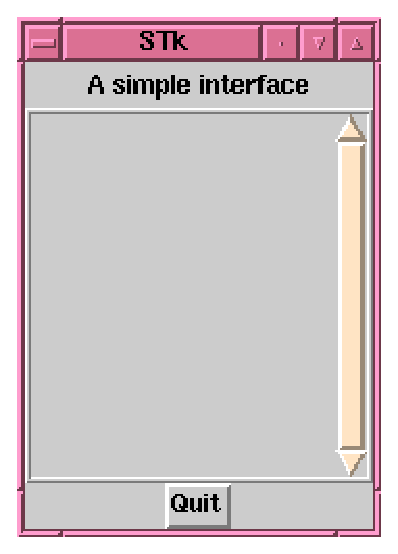
\epsfig{file=Basic-Fig-1.ps}}
\caption{A simple interface}
\label{fig-simple-interface}
\end{figure}
This interface is composed of three main components: 
\begin{enumerate}
\item a label which is situated at top
\item a frame which is itself constituted of two components: 
\begin{enumerate}
\item a listbox, and
\item a scrollbar
\end{enumerate}
\item a ``quit'' button
\end{enumerate}
Let's have look now to  the objects we'll have to create for this interface.
First we can create the top label and the quit button which are relatively
simple. This can be done with the following definitions:
\begin{quote}
\begin{verbatim}
(define lab  (make <Label>  :text "A simple interface"))
(define quit (make <Button> :text "Quit" :command '(exit)))
\end{verbatim}
\end{quote}
The {\tt :command} init-keyword permits to associate an action to the button
(this action will be triggered when the mouse button 1 will be released over
the {\tt quit} button.

The interface shown in Figure~\ref{fig-simple-interface} can be seen as a vertical alignment of
 three components (a label, a listbox with a scrollbar and a button). The
second component is itself an alignment of two object (a scrollbar and a
listbox). What is important to note here is that this alignment is an
horizontal one situated inside a vertical one. In this case, we have to place
the components of our horizontal alignment in a container which acts as a kind
of back box for further layout. The widget which permit to ``embody'' several
widgets is called a frame in the Tk toolkit. Consequently, the listbox and its
scrollbar can be defined by:
\begin{quote}
\begin{verbatim}
(define box  (make <Frame> :border-width 3 :relief "ridge"))
(define l    (make <Listbox>   :parent box))
(define s    (make <Scrollbar> :parent box :orientation "vertical"))
\end{verbatim}
\end{quote}
What is important to note is that the listbox and the scrollbar both tell that
their {\em parent} is the frame {\tt box}. This is this indication which
effectively embody them in the frame.


All the basic components of our interface have been created. What it
rests to do consists to place the graphic components we have just defined
onto screen. First we can map the listbox and its scrollbar in the {\tt
box} object with the {\em packer}\index{packer} geometry manager (see
page \pageref{pack-doc}):
\begin{quote}
\begin{verbatim}
(pack l :expand #t :fill "both" :side "left")
(pack s :expand #t :fill "y" :side "right")
\end{verbatim}
\end{quote}
Both calls to {\tt pack} permit to define the arrangement of the listbox
and the scrollbar into the frame. Here we claim that the scrollbar should
stay on the right side of the frame and that it must expand itself only in
the vertical direction if its containing frame (i.e. {\tt box}) is resized.
Concerning the listbox, it will stay on rigth and it will fill all the
space ({\tt :fill~"both"}) if {\tt box} size changes.

Now we can {\em pack} the three components of this simple interface to show
up them on screen; it can be easily done by:
\begin{quote}
\begin{verbatim}
(pack lab box quit)
\end{verbatim}
\end{quote}
The complete program for the building the previous interface is given in
Figure~\ref{simple:the_code}.

\begin{figure}
{\footnotesize
\begin{verbatim}
;;; Defining the components
(define lab  (make <Label>  :text "A simple interface"))
(define quit (make <Button> :text "Quit" :command '(exit)))
(define box  (make <Frame>  :border-width 3 :relief "ridge"))

;;; Zoom in the box
(define l    (make <Listbox>   :parent box))
(define s    (make <Scrollbar> :parent box :orientation "vertical"))

(pack l :expand #t :fill "both" :side "left")
(pack s :expand #t :fill "y" :side "right")

;;; Pack the components
(pack lab box quit)
\end{verbatim}
}
\caption{Complete code for the simple interface}
\label{simple:the_code}
\end{figure}

\subsubsection{Filling the listbox}

Filling the listbox can be done by calling the {\tt insert}
\index{listbox insert} method. This method permits to add elements in the
listbox. A way to fill the previous lisbox could be:
\begin{quote}
\begin{verbatim}
(insert l 0 "a" "b" "c")
\end{verbatim}
\end{quote}
This will insert 3 lines (containing {\tt "a"}, {\tt "b"} and {\tt "c"})
after the element whose index is 0. Inserting a {\tt "d"} between {\tt "a"}
and {\tt "b"} could be done by the following expression:
\begin{quote}
\begin{verbatim}
(insert l 1 "d")
\end{verbatim}
\end{quote}

Deleting elements of listbox necessitates a call to the {\tt delete}
method. For instance,
\begin{quote}
\begin{verbatim}
(delete l 1)
\end{verbatim}
\end{quote}
deletes the second element of the listbox (first element is at index 0), and
\begin{quote}
\begin{verbatim}
(delete l 0 2)
\end{verbatim}
\end{quote}
permits to delete the three remaining elements. 

{\tt Insert} and {\tt delete} are simple methods built upon Tk commands to
accesss listbox. Most of the time, this way of accessing a listbox is not
too convenient, and it is more easy to see the content of a listbox as its
value. Consequently, the {\tt stklos} {\tt <Listbox>} class defines a
virtual slot\cite{virtual slot} called {\tt value}\index{value} which
permits to read/fill the contents of a listbox as a {\stklos} slot.
For instance, the previous listbox can be filled with:
\begin{quote}
\begin{verbatim}
(set! (value l) '("a" "b" "c"))  ;; or (slot-set! l 'value '(...))
\end{verbatim}
\end{quote}
and the value of the second element of the listbox can be obtained by
\begin{quote}
\begin{verbatim}
(list-ref (value l) 1)
\end{verbatim}
\end{quote}

Of course, the value slot has an initialization keword associated to it,
and the filling of the listbox could have been done during the definition
of the listbox:
\begin{quote}
\begin{verbatim}
(define l (make <Listbox> :parent box 
                          :value  '("a" "b" "c")))
\end{verbatim}
\end{quote}

\subsubsection{Bringing the scrollbar to life}

For now, the lisbox and the scrollbar are disconnected (i.e. moving the
listbox, with {\tt <Shift-Button2>} doesn't move the scrollbar and clicking
the scrollbar does nothing). To make both widgets working accordingly, we have
to associate a command to each widget. First, we can associate a command to
the scrollbar, such as moving it with mouse button will move the listbox. This
can be done with:
\begin{quote}
\begin{verbatim}
(set! (command s) (format #f "y-view ~S " (address-of l)))
\end{verbatim}
\end{quote}
which associates the prefix of a Scheme command to invoke to change the view
in the listbox when the user manipulates the scrollbar. This command is
partial and will be completed effectively when the user will click the
scrollbar (see the <Scrollbar> class description on
page~\pageref{Scrollbar-class} for more details).

This is at  half way of what we have to do for cleanly associate the scrollbar
and the listbox. On the listbox side, we have to associate a command for its 
vertical movement:
\begin{quote}
\begin{verbatim}
(set! (y-scroll-command l) 
      (format #f "scrollbar-set! ~S " (address-of s)))
\end{verbatim}
\end{quote}
Here again, the command associated to the listbox is a partial since it will
be completed by Tk when needed.

As we will see in a next chapter, {\em composite widgets} will permit
to hide all this stuff, and we will be able to define a new class
which will embody a listbox and one (or two) scrollbar.

\subsection{Defining Menus}

\subsubsection{Menu-buttons and Menus}
Tk provides two widgets for building a menu: {\em menubuttons} and
{\em menus}. Those widgets are available through the {\tt
<Menu-button>} and {\tt <Menu>} classes. Instances of {\tt
<Menu-button>} class display a textual string (or a bitmap) and are
associated with an instance of the {\tt <Menu>} class.

\subsubsection{Creating a simple menu bar}

The most current task with menus concerns menu bars
building. {\stklos} provides the convenience function \Indextt{make-menubar}
to ease to the construction of menu bars. To illustrate how this
function work, we'll present the call we must write to produce the
menu bar of Figure~\ref{Menus}.
\begin{figure}
\centerline{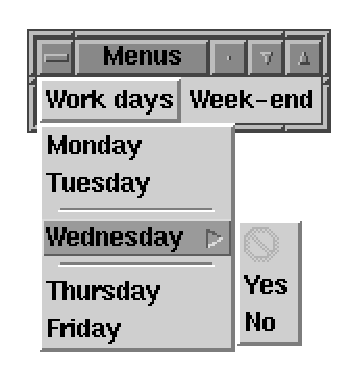
\epsfig{file=Fig2-2.eps}}
\caption{A simple menu}
\label{Menus}
\end{figure}
{\tt Make-menubar} is a function which takes a list of menu buttons
specifications. Each menu button specification is also a list.  First item
of this list is the specification of the menu button; the rest of this list
correspond to the specifaction of the menu items associated to this menu
button. To represent the menu bar of Figure\ref{Menus}, we have a
specification whih looks like:
\begin{quote}
\begin{alltt}
	((Description of {\it Work days} menu button
	     (Fisrt item of {\it Work days})
	     (Second item of {\it Work days}))
	 (Description of {\it Week end} menu button
	     (Fisrt item of {\it Week-end})
	     (Second item of {\it Week-end}))
	)
\end{alltt}
\end{quote}
The complete code for this menu bar is given in Figure\ref{Menus:code}.
Struture of menu buttons and menu items specifications is defined in
\ref{make-menubar}.
\begin{figure}
{\small
\begin{verbatim}
(define l `(("Work days" 
                 ("Monday"    ,(lambda () (format #t "Monday\n")))
                 ("Tuesday"   ,(lambda () (format #t "Tuesday\n")))
                 ("")
                 ("Wednesday"
                     ((command :bitmap error :state disabled)
                      ("Yes" ,(lambda () (format #t "Wednesday (Yes)\n")))
                      ("No"  ,(lambda () (format #t "Wednesday (No) \n")))))
                 ("")
                 ("Thursday"  ,(lambda () (format #t "Thursday\n")))
                 ("Friday"    ,(lambda () (format #t "Friday\n"))))
           ("Week-end"
                 ("Saturday"  ,(lambda () (format #t "Saturday\n")))
                 ("Sunday"    ,(lambda () (format #t "Sunday\n"))))))

(pack (make-menubar *top-root* l))
\end{verbatim}
}
\caption{Code of menu of Figure\ref{Menus}}
\label{Menus:code}
\end{figure}




\section{Simple widgets classes}
%%%%%%%%%%%%%%%%%%%%%%%%%%%%%%%%%%%%%%%%%%%%%%%%%%%%%%%%%%%%%%%%%%%%%%%%%%%%%%
% FRAME
%%%%%%%%%%%%%%%%%%%%%%%%%%%%%%%%%%%%%%%%%%%%%%%%%%%%%%%%%%%%%%%%%%%%%%%%%%%%%%

\subsection{The {\tt Frame} class}

A frame is a {\stklos} simple widget whose primary purpose is to act as a
spacer or container for complex window layouts. A frame object has several
Tk-virtual slots which are listed here:

\begin{ip}

\ITEM{background}
See section \ref{background}.

\ITEM{border-width}
See section \ref{border-width}.

\ITEM{cursor}
See section \ref{cursor}.

\ITEM{height}\label{height}
specifies the desired height for the window. This slot is only
used if the {\em geometry} slots is unspecified. If this pseudo-slot is less than 
or equal to zero (and {\em geometry} is not specified) then the window will 
not request any size at all.

\ITEM{geometry}\label{geometry}
specifies the desired geometry for the widget's window, in the
form {\em width}x{\em height}, where {\em width} is the desired
width of the window and {\em height} is the desired height.  The
units for {\em width} and {\em height} depend on the particular
widget.  For widgets displaying text the units are usually the
size of the characters in the font being displayed;  for other
widgets the units are usually pixels.

\ITEM{relief}
See section \ref{relief}.

\ITEM{width}
specifies the desired width for the window. This slot is only
used if the {\em geometry} slots is unspecified. If this pseudo-slot is less than 
or equal to zero (and {\em  geometry} is not specified) then the window will 
not request any size at all.
\end{ip}

\noindent
Furthermore, the {\em Frame} class admits a special initarg {\tt :class} which
permits to specify the new widget X11 resource class (if the {\tt :class} is
not passed as a parameter during the {\tt make-instance} of the frame, the
widget resource class will be "Frame"). The resource class of a widget can be
specified only at initialization. It can be queried by the {\tt class} reader
but cannot be changed.

Further example use a frame to group three labels in a single object. Here,
the two 
\begin{verbatim}
(setq f (make-instance 'Frame))
(setq l1 (make-instance 'Label :parent f :text " Label 1 " :relief :raised 
                               :map '(:position :left)))
(setq l2 (make-instance 'Label :parent f :text " Label 2 " :relief :raised 
                               :map '(:position :left)))
(setq l3 (make-instance 'Label :text " Label 3 " :relief :raised))
\end{verbatim}

%%%%%%%%%%%%%%%%%%%%%%%%%%%%%%%%%%%%%%%%%%%%%%%%%%%%%%%%%%%%%%%%%%%%%%%%%%%%%%
% LABEL
%%%%%%%%%%%%%%%%%%%%%%%%%%%%%%%%%%%%%%%%%%%%%%%%%%%%%%%%%%%%%%%%%%%%%%%%%%%%%%
\subsection{The label class}

The {\em Label} class defines widgets which are capable to display a textual
string or a bitmap. A label object has several pseudo-slots which are listed here:
\begin{ip}

\ITEM{anchor}\label{anchor}
specifies how the information in a widget (e.g. text or a bitmap) is to be
displayed in the widget. Must be one of the values {\em :n}, {\em :ne}, {\em
:e}, {\em :se}, {\em :s}, {\em :sw}, {\em :w}, {\em :nw}, or {\em `:center}.  For
example, {\em :nw} means display the information such that its top-left corner
is at the top-left corner of the widget.

\ITEM{background}
See section \ref{background}.

\ITEM{bitmap}\label{bitmap}
specifies a string containing the file name of the bitmap to display in the
widget. The exact way in which the bitmap is displayed may be affected by
other slots values such as {\em anchor} or {\em justify}.  Typically, if this
slot is non {\tt nil} is specified then it overrides other pseudo-slots that
specify a textual value to display in the widget; the {\em bitmap} slot may be
reset to an empty string to re-enable a text display.

\ITEM{border-width}
See section \ref{border-width}.

\ITEM{cursor}
See section \ref{cursor}.

\ITEM{font}\label{font}
specifies the font to use when drawing text inside the widget.

\ITEM{foreground}\label{foreground}
specifies the normal foreground color to use when displaying the widget.

\ITEM{height}
specifies a desired height for the label.  If a bitmap is being displayed in
the label then the value is in screen units; for text it is in lines of text.
If this pseudo-slot isn't specified, the label's desired height is computed from
the size of the bitmap or text being displayed in it.

\ITEM{pad-x}\label{pad-x}
specifies a non-negative value indicating how much extra space to request for
the widget in the X-direction. When computing how large a window it needs, the
widget will add this amount to the width it would normally need (as determined
by the width of the things displayed in the widget); if the geometry manager
can satisfy this request, the widget will end up with extra internal space to
the left and/or right of what it displays inside.

\ITEM{pad-y}\label{pad-y}
specifies a non-negative value indicating how much extra space to request for
the widget in the Y-direction. When computing how large a window it needs,
the widget will add this amount to the height it would normally need (as
determined by the height of the things displayed in the widget); if the
geometry manager can satisfy this request, the widget will end up with extra
internal space above and/or below what it displays inside.

\ITEM{relief}
See section \ref{relief}.

\ITEM{text}\label{text}
specifies a string to be displayed inside the widget.  The way in which
the string is displayed depends on the particular widget and may be
determined by other pseudo-slots, such as {\em anchor} or {\em justify}.

\ITEM{text-variable}\label{text-variable}
specifies the name of a variable. The value of the variable is a text
string to be displayed inside the widget; if the variable value changes
then the widget will automatically update itself to reflect the new value.
The way in which the string is displayed in the widget depends on the
particular widget and may be determined by other pseudo-slots, such as
{\em anchor} or {\em justify}. See below how to use this mechanism.

\ITEM{width}
Specifies a desired width for the label. If a bitmap is being displayed in
the label then the value is in screen units; for text it is in characters.  If
this pseudo-slot isn't specified, the label's desired width is computed from the
size of the bitmap or text being displayed in it.

\end{ip}

%%%%%%%%%%%%%%%%%%%%%%%%%%%%%%%%%%%%%%%%%%%%%%%%%%%%%%%%%%%%%%%%%%%%%%%%%%%%%%
% MESSAGE
%%%%%%%%%%%%%%%%%%%%%%%%%%%%%%%%%%%%%%%%%%%%%%%%%%%%%%%%%%%%%%%%%%%%%%%%%%%%%%
\section{The Message class}
The {\em Message} class defines widgets that display a textual string.  A {\em
message}widget has three special features. First, it breaks up its string into
lines in order to produce a given aspect ratio for the window.  The line
breaks are chosen at word boundaries wherever possible (if not even a single
word would fit on a line, then the word will be split across lines).  Newline
characters in the string will force line breaks; they can be used, for
example, to leave blank lines in the display.

The second feature of a message widget is justification.  The text may be
displayed left-justified, centered on a line-by-line basis, or right-justified.

The third feature of a message widget is that it handles control characters
and non-printing characters specially.  Tab characters are replaced with
enough blank space to line up on the next 8-character boundary.  Newlines
cause line breaks.  Other control characters (ASCII code less than hexadecimal
code 20) and characters not defined in the font are displayed as a
four-character sequence \\x{\it hh} where {\it hh} is the two-digit
hexadecimal number corresponding to the character.

\noindent
A message object has several pseudo-slots which are listed here:
\begin{ip}

\ITEM{anchor}
(see section \ref{anchor})

\ITEM{aspect}\label{aspect}
specifies a non-negative integer value indicating desired aspect ratio for the
text. The aspect ratio is specified as 100*width/height. 100 means the text
should be as wide as it is tall, 200 means the text should be twice as wide as
it is tall, 50 means the text should be twice as tall as it is wide, and so
on. Used to choose line length for text if {\em width} pseudo-slot isn't
specified.

\ITEM{background}
(see section \ref{background})

\ITEM{border-width}
(see section \ref{border-width})

\ITEM{cursor}
(see section \ref{cursor})

\ITEM{font}
(see section \ref{font})

\ITEM{justify}\label{justify}
specifies how to justify lines of text. Must be one of {\em :left}, {\em
:center}, or {\em :right}. Defaults to {\em left}. This pseudo-slot works
together with the {\em anchor}, {\em aspect}, {\em padX}, {\em padY}, and {\em
width} pseudo-slots to provide a variety of arrangements of the text within
the window.  The {\em aspect} and {\em width} pseudo-slots determine the
amount of screen space needed to display the text.  The {\em anchor}, {\em
padX}, and {\em padY} pseudo-slots determine where this rectangular area is
displayed within the widget's window, and the {\em justify} pseudo-slot determines
how each line is displayed within that rectangular region.  For example,
suppose {\em anchor} is {\em :e} and {\em justify} is {\em :left}, and that the
message window is much larger than needed for the text. The text will
displayed so that the left edges of all the lines line up and the right edge
of the longest line is {\em pad-x} from the right side of the window; the
entire text block will be centered in the vertical span of the window.
\ITEM{pad-x}
(see section \ref{pad-x})

\ITEM{pad-y}
(see section \ref{pad-y})

\ITEM{relief}
(see section \ref{relief})

\ITEM{text}
(see section \ref{text})

\ITEM{text-variable}
(see section \ref{text-variable})

\ITEM{width}\label{width}
specifies the length of lines in the window. If this pseudo-slot has a value
greater than zero then the {\em aspect} pseudo-slot is ignored and the {\em
width} pseudo-slot determines the line length.  If this pseudo-slot has a
value less than or equal to zero, then the {\em aspect} pseudo-slot determines
the line length.

\end {ip}

%%%%%%%%%%%%%%%%%%%%%%%%%%%%%%%%%%%%%%%%%%%%%%%%%%%%%%%%%%%%%%%%%%%%%%%%%%%%%%
% BUTTON
%%%%%%%%%%%%%%%%%%%%%%%%%%%%%%%%%%%%%%%%%%%%%%%%%%%%%%%%%%%%%%%%%%%%%%%%%%%%%%
\section{The Button class}

The {\em Button} class defines widgets that display a ``reactive'' textual
string or bitmap. It can display itself in either of three different ways,
according to the {\em state} pseudo-slot; it can be made to appear raised,
sunken, or flat; and it can be made to flash.  When a user invokes the button
(defaultly, by pressing mouse button 1 with the cursor over the button), then
the command specified in the {\em command} pseudo-slot is invoked. Several
methods are also defined for buttons. They are presented at end of chapter.

A button object has several pseudo-slots which are listed here:

\begin{ip}

\ITEM{active-background}\label{active-background}
specifies background color to use when drawing active elements.
An element (a widget or portion of a widget) is active if the
mouse cursor is positioned over the element and pressing a mouse button
will cause some action to occur.

\ITEM{active-foreground}\label{active-foreground}
specifies foreground color to use when drawing active elements.
See above for definition of active elements.

\ITEM{anchor}
(see section \ref{anchor})

\ITEM{background}
(see section \ref{background})

\ITEM{bitmap}
(see section \ref{bitmap})

\ITEM{border-width}
(see section \ref{border-width})

\ITEM{command}\label{command}
specifies a command to associate with the button. This command is typically
invoked when mouse button 1 is released over the button window.

\ITEM{cursor}
(see section \ref{cursor})

\ITEM{disabled-foreground}\label{disabled-foreground}
specifies foreground color to use when drawing a disabled element. If the
pseudo-slot is specified as an empty string (which is typically the case on
monochrome displays), disabled elements are drawn with the normal foreground
color but they are dimmed by drawing them with a stippled fill pattern.

\ITEM{font}
(see section \ref{font})

\ITEM{foreground}
(see section \ref{foreground})

\ITEM{height}
specifies a desired height for the button. If a bitmap is being displayed in
the button then the value is in screen units; for text it is in lines of text.
If this pseudo-slot isn't specified, the button's desired height is computed from
the size of the bitmap or text being displayed in it.

\ITEM{pad-x}
(see section \ref{pad-x})

\ITEM{pad-y}
(see section \ref{pad-y})

\ITEM{relief}
(see section \ref{relief})

\ITEM{state}
specifies one of three states for the button:  {\em :normal}, {\em :active},
or {\em `:disabled}.  In normal state the button is displayed using the
{\em foreground} and {\em background} pseudo-slots.  The active state is
typically used when the pointer is over the button.  In active state
the button is displayed using the {\em activeForeground} and
{\em activeBackground} pseudo-slots.  Disabled state means that the button
is insensitive:  it doesn't activate and doesn't respond to mouse
button presses.  In this state the {\em disabledForeground} and
{\em background} pseudo-slots determine how the button is displayed.

\ITEM{text}
(see section \ref{text})

\ITEM{text-variable}
(see section \ref{text-variable})

\ITEM{width}
Specifies a desired width for the button.  If a bitmap is being displayed in
the button then the value is in screen units;for text it is in characters.  If
this option isn't specified, the button's desired width is computed from the
size of the bitmap or text being displayed in it.

\end {ip}
\noindent
{\em Example}
The following example show a simple use of buttons. 
{\tt 
\begin{quote}
\begin{verbatim}
(setq b1 (make-instance 'Button :text "Yes" 
                                :command '(format t "You said Yes")))
(setq b2 (make-instance 'Button :text "No"
                                :command '(format t "You said No")))
(event-loop)
\end{verbatim}
\end{quote}}

%anchor
%background
%bitmap
%borderwidth
%cursor
%font
%foreground
%pad-x
%pad-y
%relief
%text
%text-variable

\section {Functions of this chapter}


%%%%%%%%%%%%%%%%%%%%%%%%%%%%%%%%%%%%%%%%%%%%%%%%%%%%%%%%%%%%%%%%%%%%%%%%%%%%%%
\chapter{Simple widget methods}
\section{pack}
\section{raise}
\section{lower}

%%%%%%%%%%%%%%%%%%%%%%%%%%%%%%%%%%%%%%%%%%%%%%%%%%%%%%%%%%%%%%%%%%%%%%%%%%%%%%
\chapter{The Canvas widget}

\section{The <Canvas> class}

\section{The <Canvas-item> class}
\subsection{<Rectangle> class}
\subsection{<Oval> class}

......\\
......\\
......
\section{Grouping canvas item objects}

\ldots
%%%%%%%%%%%%%%%%%%%%%%%%%%%%%%%%%%%%%%%%%%%%%%%%%%%%%%%%%%%%%%%%%%%%%%%%%%%%%%
\chapter{The Text widget}

\section{The <Text> class}
\section{The <Text-tag> class}
\section{The <Text-mark>}

%%%%%%%%%%%%%%%%%%%%%%%%%%%%%%%%%%%%%%%%%%%%%%%%%%%%%%%%%%%%%%%%%%%%%%%%%%%%%%

\chapter{Composite widgets}
\section{Standard composite widgets}

\subsection{Labeled Entry}
\subsection{Default button}
\subsection{Choice button}
\subsection{Paned window}
\subsection{Scrool Listbox}
\subsection{Scroll Text}
\subsection{Scroll Canvas}
\subsection{File box}

\section{Writing composite widgets}

%
% STklos + Tk  Documentation
%
%           Author: Erick Gallesio [eg@kaolin.unice.fr]
%    Creation date:  4-Nov-1992 15:37
% Last file update:  5-Jun-1995 14:04

\documentclass[10pt]{report}
\usepackage{a4wide}
\usepackage{alltt}
\usepackage[dvips]{epsfig}
\usepackage{fancyheadings}
\usepackage{fancybox}

\pagestyle{fancyplain}
\makeindex
\parindent0pt
\parskip2mm
\begin{document}

%
% Commands
% 

%%%% STklos
\newcommand{\stk}{{\sc STk}}
\newcommand{\stklos}{{\sc STklos}}
\newcommand{\Indextt}[1]{{\tt{#1}}\index{#1}}
\newcommand{\Index}[1]{{#1}\index{#1}}

%%%% schemetitle
%\newcommand{\schemetitle}[2]{\vbox{\vskip0.5cm\hrule\vskip10pt\noindent
%{\tt\LARGE{#1}\index{#1}}\hfill{\em{#2}}\vskip10pt\hrule}\penalty10000}

\newcommand{\schemetitle}[2]{%
\begin{center}
\vskip2mm
\Ovalbox{\parbox{0.95\textwidth}{%
\vskip1mm~~{\tt\LARGE{#1}\index{#1}}\hfill{\tt{#2}}~~\vskip1mm}}
\vskip2mm
\end{center}}


%%%% ITEM
\newcommand{\ITEM}[1]{\item[{\bf{#1}}]\index{#1}\item[]}

%
% Environments
%
%\newenvironment{schemedoc}[1]{\vskip3mm\noindent{\em #1}\samepage
%\begin{list} {} {\setlength {\rightmargin}{0cm}\setlength {\leftmargin}
%{1cm}\setlength {\topsep} {0cm}\setlength {\partopsep} {0cm}
%\setlength {\parskip} {0cm}\item}}{\end{list}}
\newenvironment{schemedoc}[1]{\vskip0mm\noindent{\em #1}
\begin{list} {} {\setlength {\rightmargin}{0cm}\setlength {\leftmargin}
{1cm}\setlength {\topsep} {0cm}\setlength {\partopsep} {0cm}
\setlength {\parskip} {0cm}\item}}{\end{list}}

%%%% ip
\newenvironment{ip}{\noindent
\begin{list} {} {\setlength {\rightmargin}{0cm}
\setlength {\leftmargin}{2cm}
\setlength {\topsep} {0cm}
\setlength {\labelsep} {0cm}
\setlength {\listparindent} {0cm}
\setlength {\partopsep} {0cm}
\setlength {\parskip} {0cm}
\item}}{\end{list}\vskip3mm}


%
% Title page
%
\thispagestyle{empty}
\begin{center}   
\ \\[3cm]
{\huge\bf Using ST{\large\bf{KLOS}} for graphic programming}\\[3mm]
{\large or}\\[4mm]
{\large\bf{``Programming the Tk toolit with an OO Scheme''}}\\[3cm]
{\large Erick Gallesio ({\tt eg\@unice\.fr})}\\
{\large\em any other volunteers are welcome}
\end{center}
\vskip10cm
\begin{flushright}
April 1995
\end{flushright}
%
% Table of content
%
\tableofcontents

%
% Chapter Getting Started
%
%           Author: Erick Gallesio [eg@kaolin.unice.fr]
%    Creation date:  4-Nov-1992 15:37
% Last file update: 24-Jul-1996 16:28

\chapter{Getting Started}

%\begin{flushright}
%{\Huge\bf 1}\\[5mm]
%{\Huge\bf Getting Started}
%\end{flushright}


This chapter will explain the things you must know to begin to manipulate Tk
widgets as {\stklos} objects. This is a short introduction for programming the
Tk toolkit with objects. If you know how to program it with the Tcl language,
you will see that things are not too much different (at least at first
sight). A good introduction to Tk programming in Tcl can be found in
\cite{Ouster-bok} or \cite{Welch-book}.

\section{First steps}

When you want to use the Tk toolkit with the {\stklos}, you must first call
the {\stk} interpreter. Launching the interpreter is usually done by a
call to the shell script {\tt stk} which must have been installed in a
standard place. Once, the interpreter is initialized, a small square window
will appear on your display. This window is called the {\em root
window\index{root window}}. Its value is always retained in the global
variable {\tt *top-root*\index{*top-root*}}.

Once the Tk initialization is complete, you have to load the file 
{\tt Tk-classes}. This can be done by 
\begin{quote}
\begin{verbatim}
(require "Tk-classes")
\end{verbatim}
\end{quote}

The {\tt Tk-classes} file contains a set of {\tt autoload}s for all the
Tk widgets defined in the {\stk} release. If you plan to always work with
those classes, you can put this line in your {\stk} init file (i.e. in the
file ``{\tt \~/.stkrc}'') to avoid (manual) loading of this file.

From now, we are able to interact with the Tk toolkit. Try to enter the following
lines at the {\stk} prompt: 
\begin{quote}
\begin{verbatim}        
(define hello (make <Label> :text "Hello, world"))
\end{verbatim}
\end{quote}

The call to {\tt make} creates a new object (i.e. an instance of the class {\tt
<Label>}) with its slot {\tt text} filled with the string {\tt "Hello,
world"}. In the above example, this new object is assigned to the symbol
{\tt hello}. Even, if a new label is created, nothing will be displayed on
your screen. You'll have to use a {\em geometry manager}\index{geometry
manager} for displaying a Tk widget onto screen. Two window managers are
provided with Tk, namely the {\em packer}\index{packer} and the {\em
placer}\index{placer}. Both command have a full set of options which will
be detailed later (see \ref{packer}). For now, we will just use the packer
in its simpler form:
\begin{quote}
\begin{verbatim}        
(pack hello)
\end{verbatim}
\end{quote}
permits to map the {\tt hello} button onto screen. 

Let us see further how the {\tt hello} button is built. Using describe
on it will display:
\begin{quote}
\begin{verbatim}
#[<label> e1444] is an instance of class <label>
Slots are: 
     id = #[Tk-command .v1]
     eid = #[Tk-command .v1]
     parent = #[Tk-command .]
     bitmap = ""
     width = 0
     height = 0
     anchor = "center"
     font = "9x15"
     foreground = "Black"
     pad-x = 1
     pad-y = 1
     text = "Hello, world"
     text-variable = ""
     background = "#cccccc"
     border-width = 0
     cursor = ""
     relief = "flat"
\end{verbatim}
\end{quote}

{\tt Id\index{Id slot}}, {\tt Eid\index{Eid slot}} and {\tt
parent\index{parent slot}} slots are present in all Tk widgets and are used
by the system. Don't try to change their value.  Other slots depend of the
kind (i.e. the class) of widget. The slots listed above correspond to
the various Tk options available on a label.  Of course you can
consult/change their value with the standard {\tt slot-ref} or {\tt
slot-set!} primitives.  For instance, one can change the background color
of the {\tt hello} button with the following form:
\begin{quote}
\begin{verbatim}
(slot-set! hello 'background "Chocolate")
\end{verbatim}
\end{quote}
or, using the {\stklos} generalized assignment,
\begin{quote}
\begin{verbatim}
(set! (background hello) "Chocolate")
\end{verbatim}
\end{quote}

Of course, the background value can be queried with
\begin{quote}
\begin{verbatim}
(slot-ref hello 'background)
        --> "Chocolate"
\end{verbatim}
\end{quote}
\noindent
or
\begin{quote}
\begin{verbatim}
(background hello)
        --> "Chocolate"
\end{verbatim}
\end{quote}

Here, {\tt background} is used as an accessor\index{accessor} of the label
background. It would be also possible to specify this value at label
instantiation with the {\tt :background} {\em initialization keyword
\index{initialization keyword}} and the same window could have be obtained
with the following {\tt make} call 
\begin{quote}
\begin{verbatim}
(define hello (make <Label> :text "Hello world" 
                            :background "Chocolate"))
\end{verbatim}
\end{quote}

\section{Class Hierarchy}

{\stklos} Tk classes permit to {\em reify} the Tk widgets into {\stklos
objects}. It means that every graphical object used in a program such as a
menu, a label or a button is represented as a {\stklos} object. All the
defined {\stklos} classes build a hierarchy which is briefly described
here. Firstly, all the classes shared a unique ancestor: the {\tt <Tk-object>}
class. Instances of this class contain informations which are necessary for
establishing a communication between the Scheme and Tk worlds. Principally,
objects of this class have the three slots cited before {\tt Id\index{Id
slot}}, {\tt Eid\index{Eid slot}} and {\tt parent\index{parent slot}}. The
{\tt Id} slot contains a Tk command \cite{STk-ref-man}, generated by
{\stklos} itself, which correspond to the {\stk} command which implement the
object.  The {\tt parent} slot contains a reference to the object which
(graphically) include the current object. This slot will be discussed later.
Normally, end users will not have to use direct instances of the {\tt
<Tk-object>} class\footnote{All classes whose name begin with the ``Tk-''
prefix are not are not intended for the final user. They will be discussed in
this document only if it seems necessary for a good class hierarchy
comprehension.}.

The next level in our class hierarchy define a fork with two branches: the
{\tt <Tk-widget>}\index{<Tk-widget> class} class and {\tt<Tk-canvas-item>}
\index{<Tk-canvas-item> class} class. Instances of the
former class are classical widgets such as buttons, menus or canvases since
instances of the later are objects contained in a canvas such as lines or
rectangles.  {\tt <Tk-widget>}s are also divided in two categories: {\tt
<Tk-simple-widget>}s and {\tt <Tk-composite-widget>}s. Simples widgets are
directly implemented as Tk objects and composite ones are build upon simple
widgets (e.g. file browser, alert messages and so on). The head of the
{\stklos} hierarchy is shown in Figure \ref{Head-hierarchy}.
\begin{figure}
%\centerline{\epsfig{figure={Fig1-1.idraw},height={2.00in},width={2.00in}}}
\centerline{\epsfig{file={Fig1-1.eps}}}
\caption{Head of the {\stklos} hierarchy}
\label{Head-hierarchy}
\end{figure}

\subsection{The {\tt <Tk-widget>} class}

No slot is defined for this class. However, since this class is common to all
the interface objects (menus, buttons, label, \ldots), it permits to define
their common behavior. The behavior of those objects is described using
{\stklos} methods with one of their argument (generally the first) which is a
{\tt <Tk-widget>}. The {\em pack\index{pack}} geometry manager cited below is
one of such methods. The {\em packer} will be fully described below (see
\pageref{packer-doc}); however, briefly stated, we can say that it permits to
explain the geometry of a widget depending of its neighbors.  The example below
shows how to use the pack primitive with arguments.
\begin{quote}
\begin{verbatim}
(define lab1 (make <Label> :text "Label 1"))
(define lab2 (make <Label> :text "Label 2"))

(pack lab1 :side "bottom")
(pack lab2 :side "top" :expand #t :fill "both")
\end{verbatim}
\end{quote}

Here, two labels are defined {\tt lab1} and {\tt lab2}. The first call to
pack says that {\tt lab1} should occupy the bottom of the window. Second
call states that {\tt lab2} will occupy the top of the window. Furthermore,
the  options {\tt :expand} and {\tt :fill} specified during {\tt lab2}
packing tells to the packer that its geometry must be adjusted to fill all
the space if its containing window is resized. If we do now 
\begin{quote}
\begin{verbatim}
(define lab3 (make <Label> :text "Label 3"))
(pack lab3 :after lab2)
\end{verbatim}
\end{quote}
we will define a new label which will be inserted between the {\tt lab1} and
{\tt lab2} labels.  Of course, the window containing the two labels  will
be {\em automagically} resized to take into account the insertion of the third.

Windows can also be unmapped from screen with the {\tt
unpack\index{unpack}} method. This method tells {\em pack} to suspend
geometry management of the specified window. Another call to a geometry
manager should be used to map again the window on display.

Suppose now that we want to delete the top most label of our previous
window (i.e. {\tt lab2}). 
This can be done with the {\tt <Tk-widget>} method {\tt destroy} as
shown below: 
\begin{quote}
\begin{verbatim}
(destroy lab2)
\end{verbatim}
\end{quote}
\noindent
Here, the window is unmapped from screen and definitively destroyed
(i.e. it cannot be mapped on the screen anymore). Technically speaking, the
widget will be destroyed and its class will be changed to the special class
{\tt <Destroyed-object>}\index{<Destroyed-object>}.

\paragraph{\bf Note:} Destroying the root window 
({\tt *top-root*\index{*top-root*}}) will destroy the root window
and, consequently, the interpreter since it as nothing more to manage.

\subsection{The {\tt <Tk-simple-widget>} class}

{\stklos} defines a class for each simple widgets (such as labels, buttons or
messages) of the Tk library. The {\tt <Tk-simple-widget>} class defines slots
and methods which are common to all those objects. The main slots defined for
simple widgets are:
\begin {ip}
\ITEM{background}\label{background}
which specifies
the normal background color to use when displaying the widget.  The value of
this slot should be a {\em string} or a {\em symbol}. It can be 
\begin{itemize}
\item a textual name
for a color defined in the server's color database file (e.g. "Chocolate" or
"Dark Olive Green").
\item a numeric specification of the red, green, and blue intensities
to use to display the color (such as {\tt \#aabbcc} or even {\tt rgb:aa/bb/cc})
using the standard X11 notation.
\end{itemize}

\ITEM{border-width}\label{border-width}
which specifies a non-negative value indicating the width of the 3-D border to
draw around the outside of the widget (if such a border is being drawn; the
{\em relief} option typically determines this).

\ITEM{cursor}\label{cursor}
which specifies the mouse
cursor to be used for the widget. Valid values for this slot are given in
Table~\ref{cursor-table}. Be aware that case is significant when naming a cursor.

\ITEM{relief}\label{relief}
which specifies the 3-D
effect desired for the widget.  Acceptable values are {\tt :raised}, {\tt
:sunken}, {\tt :flat}, {\tt :ridge} or {\tt :groove}.  The value indicates how
the interior of the widget should appear relative to its exterior; for
example, {\tt :raised} means the interior of the widget should appear to
protrude from the screen, relative to the exterior of the widget.
\end{ip}
\begin{table}
{\footnotesize
\begin{center}
\begin{tabular}{|l|l|l|l|} \hline
X\_cursor               & fleur                 & sailboat      \\
arrow                   & gobbler               & sb\_down\_arrow       \\
based\_arrow\_down      & gumby                 & sb\_h\_double\_arrow  \\
based\_arrow\_up                & hand1                 & sb\_left\_arrow       \\
boat                    & hand2                 & sb\_right\_arrow      \\
bogosity                & heart                 & sb\_up\_arrow \\
bottom\_left\_corner    & icon                  & sb\_v\_double\_arrow  \\
bottom\_right\_corner   & iron\_cross           & shuttle       \\
bottom\_side            & left\_ptr             & sizing        \\
bottom\_tee             & left\_side            & spider        \\
box\_spiral             & left\_tee             & spraycan      \\
center\_ptr             & leftbutton            & star  \\
circle                  & ll\_angle             & target        \\
clock                   & lr\_angle             & tcross        \\
coffee\_mug             & man                   & top\_left\_arrow      \\
cross                   & middlebutton          & top\_left\_corner     \\
cross\_reverse          & mouse                 & top\_right\_corner    \\
crosshair               & pencil                & top\_side     \\
diamond\_cross          & pirate                & top\_tee      \\
dot                     & plus                  & trek  \\
dotbox                  & question\_arrow       & ul\_angle     \\
double\_arrow           & right\_ptr            & umbrella      \\
draft\_large            & right\_side           & ur\_angle     \\
draft\_small            & right\_tee            & watch \\
draped\_box             & rightbutton           & xterm \\
exchange                & rtl\_logo             & {\ } \\ \hline 
\end{tabular}
\end{center}
}
\caption {Valid cursor values for slot {\tt cursor}}
\label{cursor-table}
\end{table}
These slots are defined for all the basic widgets of the {\stklos}
package. However, they are not defined as real {\stklos} slots (i.e. they are not
implanted in the Scheme world). Instead, this kind of slot has its value which
is stored inside the internal structures of the Tk library. Those slots are
allocated with a special allocation scheme which is called {\tt
:tk-virtual}. Tk virtual slots are managed by the {\tt
<With-Tk-virtual-slots-metaclass>} meta-class.

Consequently, reading or writing a {\em tk-virtual} slot will provoke a direct
reading or writing of a field of the Tk-library C-structure associated to the
object (this avoid to have to synchronize values in the Tk and Scheme
world). For each {\em tk-virtual}, {\stklos} provides an accessor; the
following example shows some simple usages of this kind of slots.

\noindent
{\em Example:}
\begin{quote}
\begin{verbatim}
(define lab (make <Label> :text "Hello" :relief "raised" :background "grey"))
(relief lab)
        --> "raised"
(set! (border-width lab) 4)
(border-width lab)
        --> 4
\end{verbatim}
\end{quote}
\noindent
The first expression creates a new instance of a label, as we have seen before. The
second one queries the Tk server about the relief of the label {\tt lab}.
Finally, the {\tt set!} expression permits to change the value of the
width of {\tt lab}'s border.

\subsection{The {\tt <Tk-canvas-item>} class}

Instances of {\tt <Tk-canvas-item>} class, as said before, are objects such as
rectangles, circles or bitmaps which are contained in a window. A window
containing this kind of object is a special simple widget called a {\em
canvas}. All the objects defined in a {\em canvas} can be manipulated
(e.g. moved, re-colored or re-sized) and even Scheme command can be associated
to them.  All the actions available for {\tt <Tk-canvas-item>}s 
are deferred to a next chapter (\ref{Canvas-chapter}).

\section{Functions of this chapter}
This section presents in details the methods and functions seen in this
chapter (or methods and functions related to things seen in this chapter).
Functions are listed below in alphabetical order.

%%%%%%%%%%%%%%%%%%%%%%%%%%%%%%%%%%%%%%%%%%%%%%%%%%%%%%%%%%%%%%%%%%%%%%%%%%%%%%
%
% DESTROY
%
%%%%%%%%%%%%%%%%%%%%%%%%%%%%%%%%%%%%%%%%%%%%%%%%%%%%%%%%%%%%%%%%%%%%%%%%%%%%%%

\label{packer-doc}
\schemetitle{destroy}{method}

\begin{schemedoc}{Syntax}
\begin{verbatim}
destroy         ((self <Tk-widget>))
destroy         l
\end{verbatim}
\end{schemedoc}

\begin{schemedoc}{Arguments (first form)}
\begin{description}
\item[self] the window to destroy.
\end{description}
\end{schemedoc}

\begin{schemedoc}{Arguments (second form)}
\begin{description}
\item[l] a list of window to destroy (this form maps in facts the previous one to
all its arguments to allow multiple destruction).
\end{description}
\end{schemedoc}

\begin{schemedoc}{Description}
{\tt Destroy} deletes the {\tt self} widget window and all of its descendants.
If {\tt self} equals to {\tt *top-root*}, the interpreter terminates its execution.
\end{schemedoc}

\begin{schemedoc}{Result}
The destroyed object (see note below)
\end{schemedoc}

\begin{schemedoc}{Example}
\begin{verbatim}
(define l1 (make <Label> :text "lab1"))
...
(define l5 (make <Label> :text "lab5"))
(destroy l1)             ;; direct call of first form
(destroy l2 l3 l4 l5)    ;; call of the second form
\end{verbatim}
\end{schemedoc}


\begin{schemedoc}{Note}
When a widget is destroyed, its class is changed to <Destroyed-object> as
shown below:
\begin{quote}
\begin{verbatim}
(define lab (make <Label> :text "A label"))
(class-name (class-of lab))
        --> <label>
(destroy lab)
(class-name (class-of lab))
        --> <destroyed-object>
\end{verbatim}
\end{quote}

\end{schemedoc}

\begin{schemedoc}{See also}
{\tt destroy} method for canvases, unpack
\end{schemedoc}

%%%%%%%%%%%%%%%%%%%%%%%%%%%%%%%%%%%%%%%%%%%%%%%%%%%%%%%%%%%%%%%%%%%%%%%%%%%%%%
%
% PACK
%
%%%%%%%%%%%%%%%%%%%%%%%%%%%%%%%%%%%%%%%%%%%%%%%%%%%%%%%%%%%%%%%%%%%%%%%%%%%%%%

\schemetitle{pack}{procedure}
\label{pack-doc}
\begin{schemedoc}{Syntax}
\begin{verbatim}
pack l 
\end{verbatim}
\end{schemedoc}

\begin{schemedoc}{Arguments}
{\tt pack} accepts a list of arguments whose behavior depends on the first
element of this list.

\paragraph{\tt (pack 'slave [slave ...] [option])}
\begin{quote}
If the first argument to {\tt pack} is a widget, then the command is
processed in the same way as {\tt (pack 'configure ...)}.
\end{quote}

\paragraph{\tt (pack 'configure [slave ...] [option])}

\begin{quote}
The arguments consist of one or more slave windows followed by pairs of
arguments that specify how to manage the slaves.  See ``THE PACKER
ALGORITHM'' below for details on how the options are used by the packer.
The following options are supported:
\begin{quote}
\par
{\tt :after  other}\\
{\tt :before other}
        \begin{quote}
                     {\tt Other} must the name of another window.   Use
                     its master as the master for the slaves, and
                     insert the slaves just after (or before)  {\tt other} 
                     in  the packing order.
        \end{quote}

\par
{\tt :anchor anchor}
        \begin{quote}
                     {\tt Anchor} must be a valid anchor position such as
                     ``{\tt n}'' or ``{\tt sw}''; it specifies where to
                     position each slave in its parcel.  Defaults to 
                     ``{\tt center}''.
        \end{quote}
\par
{\tt :expand boolean}
        \begin{quote}
                     Specifies   whether  the  slaves  should  be
                     expanded to consume  extra  space  in  their
                     master.  Defaults to {\tt \#f}.
        \end{quote}
\par
{\tt :fill style}
        \begin{quote}
         If a  slave's  parcel  is  larger  than  its
         requested  dimensions,  this  option  may be
         used to stretch the slave.  {\tt Style} must  have
         one of the following values:

         \begin{description}
          \item["none"]   Give  the slave its requested dimensions
                  plus  any  internal   padding
                 requested  with  {\tt :ipadx}  or  {\tt :ipady}.
                 This is the default.

          \item["x"]  Stretch the  slave  horizontally  to
                 fill  the entire width of its parcel
                 (except leave  external  padding  as
                 specified by {\tt :padx}).

          \item["y"]      Stretch the slave vertically to fill
                 the  entire  height  of  its  parcel
                 (except  leave  external  padding as
                 specified by {\tt :pady}).

          \item["both"]   Stretch the slave both  horizontally
                 and vertically.
         \end{description}
         \end{quote}
\par
{\tt :in other} 
        \begin{quote} 
        Insert the slave(s) at the end of the packing
        order for the master window given by other.  
        \end{quote}

\par
{\tt :ipadx amount}\\
{\tt :ipady amount}
        \begin{quote}
         {\tt Amount} specifies how much horizontal (or vertical) 
         internal padding to leave on each side of the slave(s).  
         {\tt Amount} must be a valid screen  distance, such as 2 or
         ``.5c''. It defaults to 0.
        \end{quote}

\par
{\tt :padx amount}\\
{\tt :pady amount}  
        \begin{quote}
        {\tt Amount} specifies how much horizontal external
        padding to leave on each side of the slave(s).  {\tt Amount}
        defaults to 0.
        \end{quote}

\par
{\tt :side side}
        \begin{quote}
        Specifies which side of the master the slave(s) will be packed against.
        Must be ``{\tt left}'', ``{\tt right}'', ``{\tt top}'', or ``{\tt
        bottom}''.  Defaults to ``{\tt top}''.
        \end{quote}
\end{quote}
If no {\tt :in}, {\tt :after} or {\tt :before} option is specified then
each of the slaves will be inserted at the end of the packing list for its
parent unless it is already managed by the packer (in which case it will be
left where it is).  If one of these options is specified then all the
slaves will be inserted at the specified point.  If any of the slaves are
already managed by the geometry manager then any unspecified options for
them retain their previous values rather than receiving default values.
\end{quote}

\paragraph{\tt (pack 'newinfo slave)}
\begin{quote}
Returns a list whose elements are the current configuration state of the
slave given by slave in the same option-value form that might be specified
to {\tt pack 'configure}.  The first two elements of the list are ``{\tt
-in master}'' where master is the slave's {\tt master}.  Starting with Tk
4.0 this option will be renamed ``{\tt (pack 'info ...)}''.
\end{quote}

\paragraph{\tt (pack 'propagate master [boolean])}
\begin{quote}
If {\tt boolean} is {\tt \#t} then propagation is enabled for {\tt master},
which must be a window name (see ``GEOMETRY PROPAGATION'' below).  If {\tt
boolean} has a false boolean value then propagation is disabled for {\tt
master}.  In either of these cases an empty string is returned.  If {\tt boolean}
is omitted then the command returns 0 or 1 to indicate whether propagation
is currently enabled for {\tt master}.  Propagation is enabled by default.
\end{quote}

\paragraph{\tt (pack 'slaves master)}
\begin{quote}
Returns a list of all of the slaves in the packing order for {\tt master}.
The order of the slaves in the list is the same as their order in the
packing order.  If {\tt master} has no slaves then an empty string is
returned.
\end{quote}
\end{schemedoc}

\begin{schemedoc}{Description}

{\bf THE PACKER ALGORITHM} For each master the packer maintains an ordered
list of slaves called the {\em packing list}.  The {\tt :in}, {\tt
:after}, and {\tt :before} configuration options are used to specify the
master for each slave and the slave's position in the packing list.  If
none of these options is given for a slave then the slave is added to the
end of the packing list for its parent.

The packer arranges the slaves for a master by scanning the packing list in
order.  At the time it processes each slave, a rectangular area within the
master is still unallocated.  This area is called the {\em cavity}; for the
first slave it is the entire area of the master.

For each slave the packer carries out the following steps:

\begin{enumerate}
\item
The packer allocates a rectangular {\em parcel} for the slave
along the side of the cavity given by the slave's {\tt :side} option.
If the side is top or bottom then the width of the parcel is
the width of the cavity and its height is the requested height
of the slave plus the {\tt :ipady} and {\tt :pady} options.
For the left or right side the height of the parcel is
the height of the cavity and the width is the requested width
of the slave plus the {\tt :ipadx} and {\tt :padx} options.
The parcel may be enlarged further because of the {\tt :expand}
option (see ``EXPANSION'' below)

\item
The packer chooses the dimensions of the slave.
The width will normally be the slave's requested width plus
twice its {\tt :ipadx} option and the height will normally be
the slave's requested height plus twice its {\tt :ipady}
option.
However, if the {\tt :fill} option is ``{\tt x}'' or ``{\tt both}''
then the width of the slave is expanded to fill the width of the parcel,
minus twice the {\tt :padx} option.
If the {\tt :fill} option is ``{\tt y}'' or ``{\tt both}''
then the height of the slave is expanded to fill the width of the parcel,
minus twice the {\tt :pady} option.

\item
The packer positions the slave over its parcel.
If the slave is smaller than the parcel then the {\tt :anchor}
option determines where in the parcel the slave will be placed.
If {\tt :padx} or {\tt :pady} is non-zero, then the given
amount of external padding will always be left between the
slave and the edges of the parcel.
\end{enumerate}

Once a given slave has been packed, the area of its parcel is subtracted
from the cavity, leaving a smaller rectangular cavity for the next slave.
If a slave doesn't use all of its parcel, the unused space in the parcel
will not be used by subsequent slaves.  If the cavity should become too
small to meet the needs of a slave then the slave will be given whatever
space is left in the cavity.  If the cavity shrinks to zero size, then all
remaining slaves on the packing list will be unmapped from the screen until
the master window becomes large enough to hold them again.

{\bf EXPANSION} If a master window is so large that there will be extra
space left over after all of its slaves have been packed, then the extra
space is distributed uniformly among all of the slaves for which the {\tt
:expand} option is set.  Extra horizontal space is distributed among the
expandable slaves whose {\tt :side} is ``{\tt left}'' or ``{\tt right}'',
and extra vertical space is distributed among the expandable slaves whose
{\tt :side} is ``{\tt top}'' or ``{\tt bottom}''.

{\bf GEOMETRY PROPAGATION} The packer normally computes how large a master
must be to just exactly meet the needs of its slaves, and it sets the
requested width and height of the master to these dimensions.  This causes
geometry information to propagate up through a window hierarchy to a
top-level window so that the entire sub-tree sizes itself to fit the needs
of the leaf windows.  However, the {\tt pack 'propagate} command may be used
to turn off propagation for one or more masters.  If propagation is
disabled then the packer will not set the requested width and height of the
packer.  This may be useful if, for example, you wish for a master window
to have a fixed size that you specify.

{\bf RESTRICTIONS ON MASTER WINDOWS} The master for each slave must either
be the slave's parent (the default) or a descendant of the slave's parent.
This restriction is necessary to guarantee that the slave can be placed
over any part of its master that is visible without danger of the slave
being clipped by its parent.

{\bf PACKING ORDER} If the master for a slave is not its parent then you
must make sure that the slave is higher in the stacking order than the
master.  Otherwise the master will obscure the slave and it will appear as
if the slave hasn't been packed correctly.  The easiest way to make sure
the slave is higher than the master is to create the master window first:
the most recently created window will be highest in the stacking order.
Or, you can use the {\tt raise} and {\tt lower} commands to change the
stacking order of either the master or the slave.
\end{schemedoc}

\begin{schemedoc}{Result}
None
\end{schemedoc}

\begin{schemedoc}{Example}
\begin{verbatim}
(define b1 (make <Button> :text "a button"))
(define b2 (make <Button> :text "a button with a long text"))
(define b3 (make <Button> :text "expanded button"))
(define b4 (make <Button> :text "LARGE BUTTON")) 
(pack b1 b2)
(pack b3 :expand #t :fill "x")
(pack b4 :expand #t :fill "both" :side "right" :before b1)
\end{verbatim}
These calls to {\tt pack} will produce the output shown in
Figure~\ref{pack-options}.
\end{schemedoc}
\begin{figure}
\centerline{\epsfig{file={Packing-demo.ps}}}
\caption{Using the pack options}
\label{pack-options}
\end{figure}

\begin{schemedoc}{See also}
{\tt place}, {\tt unpack}
\end{schemedoc}

%%%%%%%%%%%%%%%%%%%%%%%%%%%%%%%%%%%%%%%%%%%%%%%%%%%%%%%%%%%%%%%%%%%%%%%%%%%%%%
%
% PLACE
%
%%%%%%%%%%%%%%%%%%%%%%%%%%%%%%%%%%%%%%%%%%%%%%%%%%%%%%%%%%%%%%%%%%%%%%%%%%%%%%

\schemetitle{place}{procedure}

\begin{schemedoc}{Syntax}
\begin{verbatim}
place           l
\end{verbatim}
\end{schemedoc}

SEE TK MAN PAGE :-<

% \begin{schemedoc}{Arguments}
% \begin{description}
% \item[]
% \end{description}
% \end{schemedoc}
% 
% \begin{schemedoc}{Description}
% 
% \end{schemedoc}
% 
% \begin{schemedoc}{Result}
% 
% \end{schemedoc}
% 
% \begin{schemedoc}{Example}
% 
% \end{schemedoc}
% 
% \begin{schemedoc}{Note}
% 
% \end{schemedoc}
% 
% 
% \begin{schemedoc}{See also}
% 
% \end{schemedoc}


%%%%%%%%%%%%%%%%%%%%%%%%%%%%%%%%%%%%%%%%%%%%%%%%%%%%%%%%%%%%%%%%%%%%%%%%%%%%%%
%
% UNPACK
%
%%%%%%%%%%%%%%%%%%%%%%%%%%%%%%%%%%%%%%%%%%%%%%%%%%%%%%%%%%%%%%%%%%%%%%%%%%%%%%

\schemetitle{unpack}{procedure}

\begin{schemedoc}{Syntax}
\begin{verbatim}
unpack  l
\end{verbatim}
\end{schemedoc}

\begin{schemedoc}{Arguments}
\begin{description}
\item[l] a list of widgets to unmap.
\end{description}
\end{schemedoc}

\begin{schemedoc}{Description}
{\tt Unpack} is a simple way to unmap the widgets of the {\tt l} list. 
This procedure calls in fact {\tt pack 'forget} procedure. After the execution
of this procedure the {\em pack} geometry manager will no longer manage
the geometry of given widgets.
\end{schemedoc}

\begin{schemedoc}{Result}
Undefined
\end{schemedoc}

\begin{schemedoc}{Example}
(define l1 (make <Label> :text "lab1"))
...
(define l5 (make <Label> :text "lab5"))
(destroy l1)             ;; Object is unmapped AND destroyed
(unpack l2 l3 l4 l5)      ;; Objects are ONLY unmapped
(class-name (class-of l1))
        --> <destroyed-object>
(class-name (class-of l2))
        --> <label>
\end{schemedoc}

%\begin{schemedoc}{Note}
%
%\end{schemedoc}

\begin{schemedoc}{See also}
{\tt place}, {\tt pack}, {\tt destroy}
\end{schemedoc}
% LocalWords:  sb bogosity ptr spraycan leftbutton ll lr tcross middlebutton ul
% LocalWords:  crosshair dotbox ur rightbutton xterm rtl logo tk slave's ipadx
% LocalWords:  ipady padx pady newinfo unmap


%
% Chapter Basic
%
%           Author: Erick Gallesio [eg@kaolin.unice.fr]
%    Creation date:  6-Jan-1993 12:31
% Last file update: 20-May-1995 13:13


\chapter{Basic widgets}

This chapter is devoted to the simplest widgets of the {\stklos} package.
In fact, all the Tk widgets, except the {\em canvas} and {\em text} widgets,
are presented here.

\section{Introduction}

\subsection{A simple interface}

\subsubsection{Defining the widgets}
Before detailing all the simple widgets of the Tk library, we will see how to
build the simple interface which is shown in Figure~\ref{fig-simple-interface}. 
\begin{figure}
\centerline{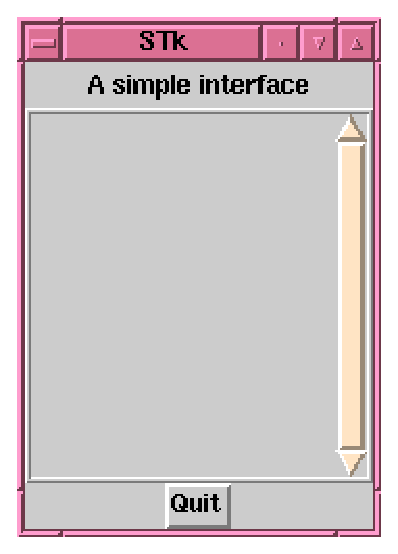
\epsfig{file=Basic-Fig-1.ps}}
\caption{A simple interface}
\label{fig-simple-interface}
\end{figure}
This interface is composed of three main components: 
\begin{enumerate}
\item a label which is situated at top
\item a frame which is itself constituted of two components: 
\begin{enumerate}
\item a listbox, and
\item a scrollbar
\end{enumerate}
\item a ``quit'' button
\end{enumerate}
Let's have look now to  the objects we'll have to create for this interface.
First we can create the top label and the quit button which are relatively
simple. This can be done with the following definitions:
\begin{quote}
\begin{verbatim}
(define lab  (make <Label>  :text "A simple interface"))
(define quit (make <Button> :text "Quit" :command '(exit)))
\end{verbatim}
\end{quote}
The {\tt :command} init-keyword permits to associate an action to the button
(this action will be triggered when the mouse button 1 will be released over
the {\tt quit} button.

The interface shown in Figure~\ref{fig-simple-interface} can be seen as a vertical alignment of
 three components (a label, a listbox with a scrollbar and a button). The
second component is itself an alignment of two object (a scrollbar and a
listbox). What is important to note here is that this alignment is an
horizontal one situated inside a vertical one. In this case, we have to place
the components of our horizontal alignment in a container which acts as a kind
of back box for further layout. The widget which permit to ``embody'' several
widgets is called a frame in the Tk toolkit. Consequently, the listbox and its
scrollbar can be defined by:
\begin{quote}
\begin{verbatim}
(define box  (make <Frame> :border-width 3 :relief "ridge"))
(define l    (make <Listbox>   :parent box))
(define s    (make <Scrollbar> :parent box :orientation "vertical"))
\end{verbatim}
\end{quote}
What is important to note is that the listbox and the scrollbar both tell that
their {\em parent} is the frame {\tt box}. This is this indication which
effectively embody them in the frame.


All the basic components of our interface have been created. What it
rests to do consists to place the graphic components we have just defined
onto screen. First we can map the listbox and its scrollbar in the {\tt
box} object with the {\em packer}\index{packer} geometry manager (see
page \pageref{pack-doc}):
\begin{quote}
\begin{verbatim}
(pack l :expand #t :fill "both" :side "left")
(pack s :expand #t :fill "y" :side "right")
\end{verbatim}
\end{quote}
Both calls to {\tt pack} permit to define the arrangement of the listbox
and the scrollbar into the frame. Here we claim that the scrollbar should
stay on the right side of the frame and that it must expand itself only in
the vertical direction if its containing frame (i.e. {\tt box}) is resized.
Concerning the listbox, it will stay on rigth and it will fill all the
space ({\tt :fill~"both"}) if {\tt box} size changes.

Now we can {\em pack} the three components of this simple interface to show
up them on screen; it can be easily done by:
\begin{quote}
\begin{verbatim}
(pack lab box quit)
\end{verbatim}
\end{quote}
The complete program for the building the previous interface is given in
Figure~\ref{simple:the_code}.

\begin{figure}
{\footnotesize
\begin{verbatim}
;;; Defining the components
(define lab  (make <Label>  :text "A simple interface"))
(define quit (make <Button> :text "Quit" :command '(exit)))
(define box  (make <Frame>  :border-width 3 :relief "ridge"))

;;; Zoom in the box
(define l    (make <Listbox>   :parent box))
(define s    (make <Scrollbar> :parent box :orientation "vertical"))

(pack l :expand #t :fill "both" :side "left")
(pack s :expand #t :fill "y" :side "right")

;;; Pack the components
(pack lab box quit)
\end{verbatim}
}
\caption{Complete code for the simple interface}
\label{simple:the_code}
\end{figure}

\subsubsection{Filling the listbox}

Filling the listbox can be done by calling the {\tt insert}
\index{listbox insert} method. This method permits to add elements in the
listbox. A way to fill the previous lisbox could be:
\begin{quote}
\begin{verbatim}
(insert l 0 "a" "b" "c")
\end{verbatim}
\end{quote}
This will insert 3 lines (containing {\tt "a"}, {\tt "b"} and {\tt "c"})
after the element whose index is 0. Inserting a {\tt "d"} between {\tt "a"}
and {\tt "b"} could be done by the following expression:
\begin{quote}
\begin{verbatim}
(insert l 1 "d")
\end{verbatim}
\end{quote}

Deleting elements of listbox necessitates a call to the {\tt delete}
method. For instance,
\begin{quote}
\begin{verbatim}
(delete l 1)
\end{verbatim}
\end{quote}
deletes the second element of the listbox (first element is at index 0), and
\begin{quote}
\begin{verbatim}
(delete l 0 2)
\end{verbatim}
\end{quote}
permits to delete the three remaining elements. 

{\tt Insert} and {\tt delete} are simple methods built upon Tk commands to
accesss listbox. Most of the time, this way of accessing a listbox is not
too convenient, and it is more easy to see the content of a listbox as its
value. Consequently, the {\tt stklos} {\tt <Listbox>} class defines a
virtual slot\cite{virtual slot} called {\tt value}\index{value} which
permits to read/fill the contents of a listbox as a {\stklos} slot.
For instance, the previous listbox can be filled with:
\begin{quote}
\begin{verbatim}
(set! (value l) '("a" "b" "c"))  ;; or (slot-set! l 'value '(...))
\end{verbatim}
\end{quote}
and the value of the second element of the listbox can be obtained by
\begin{quote}
\begin{verbatim}
(list-ref (value l) 1)
\end{verbatim}
\end{quote}

Of course, the value slot has an initialization keword associated to it,
and the filling of the listbox could have been done during the definition
of the listbox:
\begin{quote}
\begin{verbatim}
(define l (make <Listbox> :parent box 
                          :value  '("a" "b" "c")))
\end{verbatim}
\end{quote}

\subsubsection{Bringing the scrollbar to life}

For now, the lisbox and the scrollbar are disconnected (i.e. moving the
listbox, with {\tt <Shift-Button2>} doesn't move the scrollbar and clicking
the scrollbar does nothing). To make both widgets working accordingly, we have
to associate a command to each widget. First, we can associate a command to
the scrollbar, such as moving it with mouse button will move the listbox. This
can be done with:
\begin{quote}
\begin{verbatim}
(set! (command s) (format #f "y-view ~S " (address-of l)))
\end{verbatim}
\end{quote}
which associates the prefix of a Scheme command to invoke to change the view
in the listbox when the user manipulates the scrollbar. This command is
partial and will be completed effectively when the user will click the
scrollbar (see the <Scrollbar> class description on
page~\pageref{Scrollbar-class} for more details).

This is at  half way of what we have to do for cleanly associate the scrollbar
and the listbox. On the listbox side, we have to associate a command for its 
vertical movement:
\begin{quote}
\begin{verbatim}
(set! (y-scroll-command l) 
      (format #f "scrollbar-set! ~S " (address-of s)))
\end{verbatim}
\end{quote}
Here again, the command associated to the listbox is a partial since it will
be completed by Tk when needed.

As we will see in a next chapter, {\em composite widgets} will permit
to hide all this stuff, and we will be able to define a new class
which will embody a listbox and one (or two) scrollbar.

\subsection{Defining Menus}

\subsubsection{Menu-buttons and Menus}
Tk provides two widgets for building a menu: {\em menubuttons} and
{\em menus}. Those widgets are available through the {\tt
<Menu-button>} and {\tt <Menu>} classes. Instances of {\tt
<Menu-button>} class display a textual string (or a bitmap) and are
associated with an instance of the {\tt <Menu>} class.

\subsubsection{Creating a simple menu bar}

The most current task with menus concerns menu bars
building. {\stklos} provides the convenience function \Indextt{make-menubar}
to ease to the construction of menu bars. To illustrate how this
function work, we'll present the call we must write to produce the
menu bar of Figure~\ref{Menus}.
\begin{figure}
\centerline{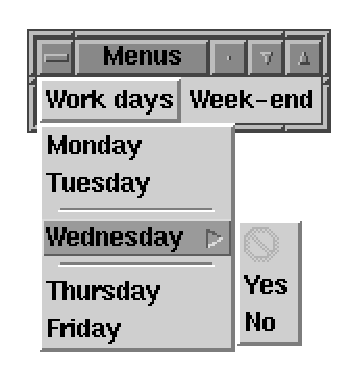
\epsfig{file=Fig2-2.eps}}
\caption{A simple menu}
\label{Menus}
\end{figure}
{\tt Make-menubar} is a function which takes a list of menu buttons
specifications. Each menu button specification is also a list.  First item
of this list is the specification of the menu button; the rest of this list
correspond to the specifaction of the menu items associated to this menu
button. To represent the menu bar of Figure\ref{Menus}, we have a
specification whih looks like:
\begin{quote}
\begin{alltt}
	((Description of {\it Work days} menu button
	     (Fisrt item of {\it Work days})
	     (Second item of {\it Work days}))
	 (Description of {\it Week end} menu button
	     (Fisrt item of {\it Week-end})
	     (Second item of {\it Week-end}))
	)
\end{alltt}
\end{quote}
The complete code for this menu bar is given in Figure\ref{Menus:code}.
Struture of menu buttons and menu items specifications is defined in
\ref{make-menubar}.
\begin{figure}
{\small
\begin{verbatim}
(define l `(("Work days" 
                 ("Monday"    ,(lambda () (format #t "Monday\n")))
                 ("Tuesday"   ,(lambda () (format #t "Tuesday\n")))
                 ("")
                 ("Wednesday"
                     ((command :bitmap error :state disabled)
                      ("Yes" ,(lambda () (format #t "Wednesday (Yes)\n")))
                      ("No"  ,(lambda () (format #t "Wednesday (No) \n")))))
                 ("")
                 ("Thursday"  ,(lambda () (format #t "Thursday\n")))
                 ("Friday"    ,(lambda () (format #t "Friday\n"))))
           ("Week-end"
                 ("Saturday"  ,(lambda () (format #t "Saturday\n")))
                 ("Sunday"    ,(lambda () (format #t "Sunday\n"))))))

(pack (make-menubar *top-root* l))
\end{verbatim}
}
\caption{Code of menu of Figure\ref{Menus}}
\label{Menus:code}
\end{figure}




\section{Simple widgets classes}
%%%%%%%%%%%%%%%%%%%%%%%%%%%%%%%%%%%%%%%%%%%%%%%%%%%%%%%%%%%%%%%%%%%%%%%%%%%%%%
% FRAME
%%%%%%%%%%%%%%%%%%%%%%%%%%%%%%%%%%%%%%%%%%%%%%%%%%%%%%%%%%%%%%%%%%%%%%%%%%%%%%

\subsection{The {\tt Frame} class}

A frame is a {\stklos} simple widget whose primary purpose is to act as a
spacer or container for complex window layouts. A frame object has several
Tk-virtual slots which are listed here:

\begin{ip}

\ITEM{background}
See section \ref{background}.

\ITEM{border-width}
See section \ref{border-width}.

\ITEM{cursor}
See section \ref{cursor}.

\ITEM{height}\label{height}
specifies the desired height for the window. This slot is only
used if the {\em geometry} slots is unspecified. If this pseudo-slot is less than 
or equal to zero (and {\em geometry} is not specified) then the window will 
not request any size at all.

\ITEM{geometry}\label{geometry}
specifies the desired geometry for the widget's window, in the
form {\em width}x{\em height}, where {\em width} is the desired
width of the window and {\em height} is the desired height.  The
units for {\em width} and {\em height} depend on the particular
widget.  For widgets displaying text the units are usually the
size of the characters in the font being displayed;  for other
widgets the units are usually pixels.

\ITEM{relief}
See section \ref{relief}.

\ITEM{width}
specifies the desired width for the window. This slot is only
used if the {\em geometry} slots is unspecified. If this pseudo-slot is less than 
or equal to zero (and {\em  geometry} is not specified) then the window will 
not request any size at all.
\end{ip}

\noindent
Furthermore, the {\em Frame} class admits a special initarg {\tt :class} which
permits to specify the new widget X11 resource class (if the {\tt :class} is
not passed as a parameter during the {\tt make-instance} of the frame, the
widget resource class will be "Frame"). The resource class of a widget can be
specified only at initialization. It can be queried by the {\tt class} reader
but cannot be changed.

Further example use a frame to group three labels in a single object. Here,
the two 
\begin{verbatim}
(setq f (make-instance 'Frame))
(setq l1 (make-instance 'Label :parent f :text " Label 1 " :relief :raised 
                               :map '(:position :left)))
(setq l2 (make-instance 'Label :parent f :text " Label 2 " :relief :raised 
                               :map '(:position :left)))
(setq l3 (make-instance 'Label :text " Label 3 " :relief :raised))
\end{verbatim}

%%%%%%%%%%%%%%%%%%%%%%%%%%%%%%%%%%%%%%%%%%%%%%%%%%%%%%%%%%%%%%%%%%%%%%%%%%%%%%
% LABEL
%%%%%%%%%%%%%%%%%%%%%%%%%%%%%%%%%%%%%%%%%%%%%%%%%%%%%%%%%%%%%%%%%%%%%%%%%%%%%%
\subsection{The label class}

The {\em Label} class defines widgets which are capable to display a textual
string or a bitmap. A label object has several pseudo-slots which are listed here:
\begin{ip}

\ITEM{anchor}\label{anchor}
specifies how the information in a widget (e.g. text or a bitmap) is to be
displayed in the widget. Must be one of the values {\em :n}, {\em :ne}, {\em
:e}, {\em :se}, {\em :s}, {\em :sw}, {\em :w}, {\em :nw}, or {\em `:center}.  For
example, {\em :nw} means display the information such that its top-left corner
is at the top-left corner of the widget.

\ITEM{background}
See section \ref{background}.

\ITEM{bitmap}\label{bitmap}
specifies a string containing the file name of the bitmap to display in the
widget. The exact way in which the bitmap is displayed may be affected by
other slots values such as {\em anchor} or {\em justify}.  Typically, if this
slot is non {\tt nil} is specified then it overrides other pseudo-slots that
specify a textual value to display in the widget; the {\em bitmap} slot may be
reset to an empty string to re-enable a text display.

\ITEM{border-width}
See section \ref{border-width}.

\ITEM{cursor}
See section \ref{cursor}.

\ITEM{font}\label{font}
specifies the font to use when drawing text inside the widget.

\ITEM{foreground}\label{foreground}
specifies the normal foreground color to use when displaying the widget.

\ITEM{height}
specifies a desired height for the label.  If a bitmap is being displayed in
the label then the value is in screen units; for text it is in lines of text.
If this pseudo-slot isn't specified, the label's desired height is computed from
the size of the bitmap or text being displayed in it.

\ITEM{pad-x}\label{pad-x}
specifies a non-negative value indicating how much extra space to request for
the widget in the X-direction. When computing how large a window it needs, the
widget will add this amount to the width it would normally need (as determined
by the width of the things displayed in the widget); if the geometry manager
can satisfy this request, the widget will end up with extra internal space to
the left and/or right of what it displays inside.

\ITEM{pad-y}\label{pad-y}
specifies a non-negative value indicating how much extra space to request for
the widget in the Y-direction. When computing how large a window it needs,
the widget will add this amount to the height it would normally need (as
determined by the height of the things displayed in the widget); if the
geometry manager can satisfy this request, the widget will end up with extra
internal space above and/or below what it displays inside.

\ITEM{relief}
See section \ref{relief}.

\ITEM{text}\label{text}
specifies a string to be displayed inside the widget.  The way in which
the string is displayed depends on the particular widget and may be
determined by other pseudo-slots, such as {\em anchor} or {\em justify}.

\ITEM{text-variable}\label{text-variable}
specifies the name of a variable. The value of the variable is a text
string to be displayed inside the widget; if the variable value changes
then the widget will automatically update itself to reflect the new value.
The way in which the string is displayed in the widget depends on the
particular widget and may be determined by other pseudo-slots, such as
{\em anchor} or {\em justify}. See below how to use this mechanism.

\ITEM{width}
Specifies a desired width for the label. If a bitmap is being displayed in
the label then the value is in screen units; for text it is in characters.  If
this pseudo-slot isn't specified, the label's desired width is computed from the
size of the bitmap or text being displayed in it.

\end{ip}

%%%%%%%%%%%%%%%%%%%%%%%%%%%%%%%%%%%%%%%%%%%%%%%%%%%%%%%%%%%%%%%%%%%%%%%%%%%%%%
% MESSAGE
%%%%%%%%%%%%%%%%%%%%%%%%%%%%%%%%%%%%%%%%%%%%%%%%%%%%%%%%%%%%%%%%%%%%%%%%%%%%%%
\section{The Message class}
The {\em Message} class defines widgets that display a textual string.  A {\em
message}widget has three special features. First, it breaks up its string into
lines in order to produce a given aspect ratio for the window.  The line
breaks are chosen at word boundaries wherever possible (if not even a single
word would fit on a line, then the word will be split across lines).  Newline
characters in the string will force line breaks; they can be used, for
example, to leave blank lines in the display.

The second feature of a message widget is justification.  The text may be
displayed left-justified, centered on a line-by-line basis, or right-justified.

The third feature of a message widget is that it handles control characters
and non-printing characters specially.  Tab characters are replaced with
enough blank space to line up on the next 8-character boundary.  Newlines
cause line breaks.  Other control characters (ASCII code less than hexadecimal
code 20) and characters not defined in the font are displayed as a
four-character sequence \\x{\it hh} where {\it hh} is the two-digit
hexadecimal number corresponding to the character.

\noindent
A message object has several pseudo-slots which are listed here:
\begin{ip}

\ITEM{anchor}
(see section \ref{anchor})

\ITEM{aspect}\label{aspect}
specifies a non-negative integer value indicating desired aspect ratio for the
text. The aspect ratio is specified as 100*width/height. 100 means the text
should be as wide as it is tall, 200 means the text should be twice as wide as
it is tall, 50 means the text should be twice as tall as it is wide, and so
on. Used to choose line length for text if {\em width} pseudo-slot isn't
specified.

\ITEM{background}
(see section \ref{background})

\ITEM{border-width}
(see section \ref{border-width})

\ITEM{cursor}
(see section \ref{cursor})

\ITEM{font}
(see section \ref{font})

\ITEM{justify}\label{justify}
specifies how to justify lines of text. Must be one of {\em :left}, {\em
:center}, or {\em :right}. Defaults to {\em left}. This pseudo-slot works
together with the {\em anchor}, {\em aspect}, {\em padX}, {\em padY}, and {\em
width} pseudo-slots to provide a variety of arrangements of the text within
the window.  The {\em aspect} and {\em width} pseudo-slots determine the
amount of screen space needed to display the text.  The {\em anchor}, {\em
padX}, and {\em padY} pseudo-slots determine where this rectangular area is
displayed within the widget's window, and the {\em justify} pseudo-slot determines
how each line is displayed within that rectangular region.  For example,
suppose {\em anchor} is {\em :e} and {\em justify} is {\em :left}, and that the
message window is much larger than needed for the text. The text will
displayed so that the left edges of all the lines line up and the right edge
of the longest line is {\em pad-x} from the right side of the window; the
entire text block will be centered in the vertical span of the window.
\ITEM{pad-x}
(see section \ref{pad-x})

\ITEM{pad-y}
(see section \ref{pad-y})

\ITEM{relief}
(see section \ref{relief})

\ITEM{text}
(see section \ref{text})

\ITEM{text-variable}
(see section \ref{text-variable})

\ITEM{width}\label{width}
specifies the length of lines in the window. If this pseudo-slot has a value
greater than zero then the {\em aspect} pseudo-slot is ignored and the {\em
width} pseudo-slot determines the line length.  If this pseudo-slot has a
value less than or equal to zero, then the {\em aspect} pseudo-slot determines
the line length.

\end {ip}

%%%%%%%%%%%%%%%%%%%%%%%%%%%%%%%%%%%%%%%%%%%%%%%%%%%%%%%%%%%%%%%%%%%%%%%%%%%%%%
% BUTTON
%%%%%%%%%%%%%%%%%%%%%%%%%%%%%%%%%%%%%%%%%%%%%%%%%%%%%%%%%%%%%%%%%%%%%%%%%%%%%%
\section{The Button class}

The {\em Button} class defines widgets that display a ``reactive'' textual
string or bitmap. It can display itself in either of three different ways,
according to the {\em state} pseudo-slot; it can be made to appear raised,
sunken, or flat; and it can be made to flash.  When a user invokes the button
(defaultly, by pressing mouse button 1 with the cursor over the button), then
the command specified in the {\em command} pseudo-slot is invoked. Several
methods are also defined for buttons. They are presented at end of chapter.

A button object has several pseudo-slots which are listed here:

\begin{ip}

\ITEM{active-background}\label{active-background}
specifies background color to use when drawing active elements.
An element (a widget or portion of a widget) is active if the
mouse cursor is positioned over the element and pressing a mouse button
will cause some action to occur.

\ITEM{active-foreground}\label{active-foreground}
specifies foreground color to use when drawing active elements.
See above for definition of active elements.

\ITEM{anchor}
(see section \ref{anchor})

\ITEM{background}
(see section \ref{background})

\ITEM{bitmap}
(see section \ref{bitmap})

\ITEM{border-width}
(see section \ref{border-width})

\ITEM{command}\label{command}
specifies a command to associate with the button. This command is typically
invoked when mouse button 1 is released over the button window.

\ITEM{cursor}
(see section \ref{cursor})

\ITEM{disabled-foreground}\label{disabled-foreground}
specifies foreground color to use when drawing a disabled element. If the
pseudo-slot is specified as an empty string (which is typically the case on
monochrome displays), disabled elements are drawn with the normal foreground
color but they are dimmed by drawing them with a stippled fill pattern.

\ITEM{font}
(see section \ref{font})

\ITEM{foreground}
(see section \ref{foreground})

\ITEM{height}
specifies a desired height for the button. If a bitmap is being displayed in
the button then the value is in screen units; for text it is in lines of text.
If this pseudo-slot isn't specified, the button's desired height is computed from
the size of the bitmap or text being displayed in it.

\ITEM{pad-x}
(see section \ref{pad-x})

\ITEM{pad-y}
(see section \ref{pad-y})

\ITEM{relief}
(see section \ref{relief})

\ITEM{state}
specifies one of three states for the button:  {\em :normal}, {\em :active},
or {\em `:disabled}.  In normal state the button is displayed using the
{\em foreground} and {\em background} pseudo-slots.  The active state is
typically used when the pointer is over the button.  In active state
the button is displayed using the {\em activeForeground} and
{\em activeBackground} pseudo-slots.  Disabled state means that the button
is insensitive:  it doesn't activate and doesn't respond to mouse
button presses.  In this state the {\em disabledForeground} and
{\em background} pseudo-slots determine how the button is displayed.

\ITEM{text}
(see section \ref{text})

\ITEM{text-variable}
(see section \ref{text-variable})

\ITEM{width}
Specifies a desired width for the button.  If a bitmap is being displayed in
the button then the value is in screen units;for text it is in characters.  If
this option isn't specified, the button's desired width is computed from the
size of the bitmap or text being displayed in it.

\end {ip}
\noindent
{\em Example}
The following example show a simple use of buttons. 
{\tt 
\begin{quote}
\begin{verbatim}
(setq b1 (make-instance 'Button :text "Yes" 
                                :command '(format t "You said Yes")))
(setq b2 (make-instance 'Button :text "No"
                                :command '(format t "You said No")))
(event-loop)
\end{verbatim}
\end{quote}}

%anchor
%background
%bitmap
%borderwidth
%cursor
%font
%foreground
%pad-x
%pad-y
%relief
%text
%text-variable

\section {Functions of this chapter}


%%%%%%%%%%%%%%%%%%%%%%%%%%%%%%%%%%%%%%%%%%%%%%%%%%%%%%%%%%%%%%%%%%%%%%%%%%%%%%
\chapter{Simple widget methods}
\section{pack}
\section{raise}
\section{lower}

%%%%%%%%%%%%%%%%%%%%%%%%%%%%%%%%%%%%%%%%%%%%%%%%%%%%%%%%%%%%%%%%%%%%%%%%%%%%%%
\chapter{The Canvas widget}

\section{The <Canvas> class}

\section{The <Canvas-item> class}
\subsection{<Rectangle> class}
\subsection{<Oval> class}

......\\
......\\
......
\section{Grouping canvas item objects}

\ldots
%%%%%%%%%%%%%%%%%%%%%%%%%%%%%%%%%%%%%%%%%%%%%%%%%%%%%%%%%%%%%%%%%%%%%%%%%%%%%%
\chapter{The Text widget}

\section{The <Text> class}
\section{The <Text-tag> class}
\section{The <Text-mark>}

%%%%%%%%%%%%%%%%%%%%%%%%%%%%%%%%%%%%%%%%%%%%%%%%%%%%%%%%%%%%%%%%%%%%%%%%%%%%%%

\chapter{Composite widgets}
\section{Standard composite widgets}

\subsection{Labeled Entry}
\subsection{Default button}
\subsection{Choice button}
\subsection{Paned window}
\subsection{Scrool Listbox}
\subsection{Scroll Text}
\subsection{Scroll Canvas}
\subsection{File box}

\section{Writing composite widgets}

%
% STklos + Tk  Documentation
%
%           Author: Erick Gallesio [eg@kaolin.unice.fr]
%    Creation date:  4-Nov-1992 15:37
% Last file update:  5-Jun-1995 14:04

\documentclass[10pt]{report}
\usepackage{a4wide}
\usepackage{alltt}
\usepackage[dvips]{epsfig}
\usepackage{fancyheadings}
\usepackage{fancybox}

\pagestyle{fancyplain}
\makeindex
\parindent0pt
\parskip2mm
\begin{document}

%
% Commands
% 

%%%% STklos
\newcommand{\stk}{{\sc STk}}
\newcommand{\stklos}{{\sc STklos}}
\newcommand{\Indextt}[1]{{\tt{#1}}\index{#1}}
\newcommand{\Index}[1]{{#1}\index{#1}}

%%%% schemetitle
%\newcommand{\schemetitle}[2]{\vbox{\vskip0.5cm\hrule\vskip10pt\noindent
%{\tt\LARGE{#1}\index{#1}}\hfill{\em{#2}}\vskip10pt\hrule}\penalty10000}

\newcommand{\schemetitle}[2]{%
\begin{center}
\vskip2mm
\Ovalbox{\parbox{0.95\textwidth}{%
\vskip1mm~~{\tt\LARGE{#1}\index{#1}}\hfill{\tt{#2}}~~\vskip1mm}}
\vskip2mm
\end{center}}


%%%% ITEM
\newcommand{\ITEM}[1]{\item[{\bf{#1}}]\index{#1}\item[]}

%
% Environments
%
%\newenvironment{schemedoc}[1]{\vskip3mm\noindent{\em #1}\samepage
%\begin{list} {} {\setlength {\rightmargin}{0cm}\setlength {\leftmargin}
%{1cm}\setlength {\topsep} {0cm}\setlength {\partopsep} {0cm}
%\setlength {\parskip} {0cm}\item}}{\end{list}}
\newenvironment{schemedoc}[1]{\vskip0mm\noindent{\em #1}
\begin{list} {} {\setlength {\rightmargin}{0cm}\setlength {\leftmargin}
{1cm}\setlength {\topsep} {0cm}\setlength {\partopsep} {0cm}
\setlength {\parskip} {0cm}\item}}{\end{list}}

%%%% ip
\newenvironment{ip}{\noindent
\begin{list} {} {\setlength {\rightmargin}{0cm}
\setlength {\leftmargin}{2cm}
\setlength {\topsep} {0cm}
\setlength {\labelsep} {0cm}
\setlength {\listparindent} {0cm}
\setlength {\partopsep} {0cm}
\setlength {\parskip} {0cm}
\item}}{\end{list}\vskip3mm}


%
% Title page
%
\thispagestyle{empty}
\begin{center}   
\ \\[3cm]
{\huge\bf Using ST{\large\bf{KLOS}} for graphic programming}\\[3mm]
{\large or}\\[4mm]
{\large\bf{``Programming the Tk toolit with an OO Scheme''}}\\[3cm]
{\large Erick Gallesio ({\tt eg\@unice\.fr})}\\
{\large\em any other volunteers are welcome}
\end{center}
\vskip10cm
\begin{flushright}
April 1995
\end{flushright}
%
% Table of content
%
\tableofcontents

%
% Chapter Getting Started
%
%           Author: Erick Gallesio [eg@kaolin.unice.fr]
%    Creation date:  4-Nov-1992 15:37
% Last file update: 24-Jul-1996 16:28

\chapter{Getting Started}

%\begin{flushright}
%{\Huge\bf 1}\\[5mm]
%{\Huge\bf Getting Started}
%\end{flushright}


This chapter will explain the things you must know to begin to manipulate Tk
widgets as {\stklos} objects. This is a short introduction for programming the
Tk toolkit with objects. If you know how to program it with the Tcl language,
you will see that things are not too much different (at least at first
sight). A good introduction to Tk programming in Tcl can be found in
\cite{Ouster-bok} or \cite{Welch-book}.

\section{First steps}

When you want to use the Tk toolkit with the {\stklos}, you must first call
the {\stk} interpreter. Launching the interpreter is usually done by a
call to the shell script {\tt stk} which must have been installed in a
standard place. Once, the interpreter is initialized, a small square window
will appear on your display. This window is called the {\em root
window\index{root window}}. Its value is always retained in the global
variable {\tt *top-root*\index{*top-root*}}.

Once the Tk initialization is complete, you have to load the file 
{\tt Tk-classes}. This can be done by 
\begin{quote}
\begin{verbatim}
(require "Tk-classes")
\end{verbatim}
\end{quote}

The {\tt Tk-classes} file contains a set of {\tt autoload}s for all the
Tk widgets defined in the {\stk} release. If you plan to always work with
those classes, you can put this line in your {\stk} init file (i.e. in the
file ``{\tt \~/.stkrc}'') to avoid (manual) loading of this file.

From now, we are able to interact with the Tk toolkit. Try to enter the following
lines at the {\stk} prompt: 
\begin{quote}
\begin{verbatim}        
(define hello (make <Label> :text "Hello, world"))
\end{verbatim}
\end{quote}

The call to {\tt make} creates a new object (i.e. an instance of the class {\tt
<Label>}) with its slot {\tt text} filled with the string {\tt "Hello,
world"}. In the above example, this new object is assigned to the symbol
{\tt hello}. Even, if a new label is created, nothing will be displayed on
your screen. You'll have to use a {\em geometry manager}\index{geometry
manager} for displaying a Tk widget onto screen. Two window managers are
provided with Tk, namely the {\em packer}\index{packer} and the {\em
placer}\index{placer}. Both command have a full set of options which will
be detailed later (see \ref{packer}). For now, we will just use the packer
in its simpler form:
\begin{quote}
\begin{verbatim}        
(pack hello)
\end{verbatim}
\end{quote}
permits to map the {\tt hello} button onto screen. 

Let us see further how the {\tt hello} button is built. Using describe
on it will display:
\begin{quote}
\begin{verbatim}
#[<label> e1444] is an instance of class <label>
Slots are: 
     id = #[Tk-command .v1]
     eid = #[Tk-command .v1]
     parent = #[Tk-command .]
     bitmap = ""
     width = 0
     height = 0
     anchor = "center"
     font = "9x15"
     foreground = "Black"
     pad-x = 1
     pad-y = 1
     text = "Hello, world"
     text-variable = ""
     background = "#cccccc"
     border-width = 0
     cursor = ""
     relief = "flat"
\end{verbatim}
\end{quote}

{\tt Id\index{Id slot}}, {\tt Eid\index{Eid slot}} and {\tt
parent\index{parent slot}} slots are present in all Tk widgets and are used
by the system. Don't try to change their value.  Other slots depend of the
kind (i.e. the class) of widget. The slots listed above correspond to
the various Tk options available on a label.  Of course you can
consult/change their value with the standard {\tt slot-ref} or {\tt
slot-set!} primitives.  For instance, one can change the background color
of the {\tt hello} button with the following form:
\begin{quote}
\begin{verbatim}
(slot-set! hello 'background "Chocolate")
\end{verbatim}
\end{quote}
or, using the {\stklos} generalized assignment,
\begin{quote}
\begin{verbatim}
(set! (background hello) "Chocolate")
\end{verbatim}
\end{quote}

Of course, the background value can be queried with
\begin{quote}
\begin{verbatim}
(slot-ref hello 'background)
        --> "Chocolate"
\end{verbatim}
\end{quote}
\noindent
or
\begin{quote}
\begin{verbatim}
(background hello)
        --> "Chocolate"
\end{verbatim}
\end{quote}

Here, {\tt background} is used as an accessor\index{accessor} of the label
background. It would be also possible to specify this value at label
instantiation with the {\tt :background} {\em initialization keyword
\index{initialization keyword}} and the same window could have be obtained
with the following {\tt make} call 
\begin{quote}
\begin{verbatim}
(define hello (make <Label> :text "Hello world" 
                            :background "Chocolate"))
\end{verbatim}
\end{quote}

\section{Class Hierarchy}

{\stklos} Tk classes permit to {\em reify} the Tk widgets into {\stklos
objects}. It means that every graphical object used in a program such as a
menu, a label or a button is represented as a {\stklos} object. All the
defined {\stklos} classes build a hierarchy which is briefly described
here. Firstly, all the classes shared a unique ancestor: the {\tt <Tk-object>}
class. Instances of this class contain informations which are necessary for
establishing a communication between the Scheme and Tk worlds. Principally,
objects of this class have the three slots cited before {\tt Id\index{Id
slot}}, {\tt Eid\index{Eid slot}} and {\tt parent\index{parent slot}}. The
{\tt Id} slot contains a Tk command \cite{STk-ref-man}, generated by
{\stklos} itself, which correspond to the {\stk} command which implement the
object.  The {\tt parent} slot contains a reference to the object which
(graphically) include the current object. This slot will be discussed later.
Normally, end users will not have to use direct instances of the {\tt
<Tk-object>} class\footnote{All classes whose name begin with the ``Tk-''
prefix are not are not intended for the final user. They will be discussed in
this document only if it seems necessary for a good class hierarchy
comprehension.}.

The next level in our class hierarchy define a fork with two branches: the
{\tt <Tk-widget>}\index{<Tk-widget> class} class and {\tt<Tk-canvas-item>}
\index{<Tk-canvas-item> class} class. Instances of the
former class are classical widgets such as buttons, menus or canvases since
instances of the later are objects contained in a canvas such as lines or
rectangles.  {\tt <Tk-widget>}s are also divided in two categories: {\tt
<Tk-simple-widget>}s and {\tt <Tk-composite-widget>}s. Simples widgets are
directly implemented as Tk objects and composite ones are build upon simple
widgets (e.g. file browser, alert messages and so on). The head of the
{\stklos} hierarchy is shown in Figure \ref{Head-hierarchy}.
\begin{figure}
%\centerline{\epsfig{figure={Fig1-1.idraw},height={2.00in},width={2.00in}}}
\centerline{\epsfig{file={Fig1-1.eps}}}
\caption{Head of the {\stklos} hierarchy}
\label{Head-hierarchy}
\end{figure}

\subsection{The {\tt <Tk-widget>} class}

No slot is defined for this class. However, since this class is common to all
the interface objects (menus, buttons, label, \ldots), it permits to define
their common behavior. The behavior of those objects is described using
{\stklos} methods with one of their argument (generally the first) which is a
{\tt <Tk-widget>}. The {\em pack\index{pack}} geometry manager cited below is
one of such methods. The {\em packer} will be fully described below (see
\pageref{packer-doc}); however, briefly stated, we can say that it permits to
explain the geometry of a widget depending of its neighbors.  The example below
shows how to use the pack primitive with arguments.
\begin{quote}
\begin{verbatim}
(define lab1 (make <Label> :text "Label 1"))
(define lab2 (make <Label> :text "Label 2"))

(pack lab1 :side "bottom")
(pack lab2 :side "top" :expand #t :fill "both")
\end{verbatim}
\end{quote}

Here, two labels are defined {\tt lab1} and {\tt lab2}. The first call to
pack says that {\tt lab1} should occupy the bottom of the window. Second
call states that {\tt lab2} will occupy the top of the window. Furthermore,
the  options {\tt :expand} and {\tt :fill} specified during {\tt lab2}
packing tells to the packer that its geometry must be adjusted to fill all
the space if its containing window is resized. If we do now 
\begin{quote}
\begin{verbatim}
(define lab3 (make <Label> :text "Label 3"))
(pack lab3 :after lab2)
\end{verbatim}
\end{quote}
we will define a new label which will be inserted between the {\tt lab1} and
{\tt lab2} labels.  Of course, the window containing the two labels  will
be {\em automagically} resized to take into account the insertion of the third.

Windows can also be unmapped from screen with the {\tt
unpack\index{unpack}} method. This method tells {\em pack} to suspend
geometry management of the specified window. Another call to a geometry
manager should be used to map again the window on display.

Suppose now that we want to delete the top most label of our previous
window (i.e. {\tt lab2}). 
This can be done with the {\tt <Tk-widget>} method {\tt destroy} as
shown below: 
\begin{quote}
\begin{verbatim}
(destroy lab2)
\end{verbatim}
\end{quote}
\noindent
Here, the window is unmapped from screen and definitively destroyed
(i.e. it cannot be mapped on the screen anymore). Technically speaking, the
widget will be destroyed and its class will be changed to the special class
{\tt <Destroyed-object>}\index{<Destroyed-object>}.

\paragraph{\bf Note:} Destroying the root window 
({\tt *top-root*\index{*top-root*}}) will destroy the root window
and, consequently, the interpreter since it as nothing more to manage.

\subsection{The {\tt <Tk-simple-widget>} class}

{\stklos} defines a class for each simple widgets (such as labels, buttons or
messages) of the Tk library. The {\tt <Tk-simple-widget>} class defines slots
and methods which are common to all those objects. The main slots defined for
simple widgets are:
\begin {ip}
\ITEM{background}\label{background}
which specifies
the normal background color to use when displaying the widget.  The value of
this slot should be a {\em string} or a {\em symbol}. It can be 
\begin{itemize}
\item a textual name
for a color defined in the server's color database file (e.g. "Chocolate" or
"Dark Olive Green").
\item a numeric specification of the red, green, and blue intensities
to use to display the color (such as {\tt \#aabbcc} or even {\tt rgb:aa/bb/cc})
using the standard X11 notation.
\end{itemize}

\ITEM{border-width}\label{border-width}
which specifies a non-negative value indicating the width of the 3-D border to
draw around the outside of the widget (if such a border is being drawn; the
{\em relief} option typically determines this).

\ITEM{cursor}\label{cursor}
which specifies the mouse
cursor to be used for the widget. Valid values for this slot are given in
Table~\ref{cursor-table}. Be aware that case is significant when naming a cursor.

\ITEM{relief}\label{relief}
which specifies the 3-D
effect desired for the widget.  Acceptable values are {\tt :raised}, {\tt
:sunken}, {\tt :flat}, {\tt :ridge} or {\tt :groove}.  The value indicates how
the interior of the widget should appear relative to its exterior; for
example, {\tt :raised} means the interior of the widget should appear to
protrude from the screen, relative to the exterior of the widget.
\end{ip}
\begin{table}
{\footnotesize
\begin{center}
\begin{tabular}{|l|l|l|l|} \hline
X\_cursor               & fleur                 & sailboat      \\
arrow                   & gobbler               & sb\_down\_arrow       \\
based\_arrow\_down      & gumby                 & sb\_h\_double\_arrow  \\
based\_arrow\_up                & hand1                 & sb\_left\_arrow       \\
boat                    & hand2                 & sb\_right\_arrow      \\
bogosity                & heart                 & sb\_up\_arrow \\
bottom\_left\_corner    & icon                  & sb\_v\_double\_arrow  \\
bottom\_right\_corner   & iron\_cross           & shuttle       \\
bottom\_side            & left\_ptr             & sizing        \\
bottom\_tee             & left\_side            & spider        \\
box\_spiral             & left\_tee             & spraycan      \\
center\_ptr             & leftbutton            & star  \\
circle                  & ll\_angle             & target        \\
clock                   & lr\_angle             & tcross        \\
coffee\_mug             & man                   & top\_left\_arrow      \\
cross                   & middlebutton          & top\_left\_corner     \\
cross\_reverse          & mouse                 & top\_right\_corner    \\
crosshair               & pencil                & top\_side     \\
diamond\_cross          & pirate                & top\_tee      \\
dot                     & plus                  & trek  \\
dotbox                  & question\_arrow       & ul\_angle     \\
double\_arrow           & right\_ptr            & umbrella      \\
draft\_large            & right\_side           & ur\_angle     \\
draft\_small            & right\_tee            & watch \\
draped\_box             & rightbutton           & xterm \\
exchange                & rtl\_logo             & {\ } \\ \hline 
\end{tabular}
\end{center}
}
\caption {Valid cursor values for slot {\tt cursor}}
\label{cursor-table}
\end{table}
These slots are defined for all the basic widgets of the {\stklos}
package. However, they are not defined as real {\stklos} slots (i.e. they are not
implanted in the Scheme world). Instead, this kind of slot has its value which
is stored inside the internal structures of the Tk library. Those slots are
allocated with a special allocation scheme which is called {\tt
:tk-virtual}. Tk virtual slots are managed by the {\tt
<With-Tk-virtual-slots-metaclass>} meta-class.

Consequently, reading or writing a {\em tk-virtual} slot will provoke a direct
reading or writing of a field of the Tk-library C-structure associated to the
object (this avoid to have to synchronize values in the Tk and Scheme
world). For each {\em tk-virtual}, {\stklos} provides an accessor; the
following example shows some simple usages of this kind of slots.

\noindent
{\em Example:}
\begin{quote}
\begin{verbatim}
(define lab (make <Label> :text "Hello" :relief "raised" :background "grey"))
(relief lab)
        --> "raised"
(set! (border-width lab) 4)
(border-width lab)
        --> 4
\end{verbatim}
\end{quote}
\noindent
The first expression creates a new instance of a label, as we have seen before. The
second one queries the Tk server about the relief of the label {\tt lab}.
Finally, the {\tt set!} expression permits to change the value of the
width of {\tt lab}'s border.

\subsection{The {\tt <Tk-canvas-item>} class}

Instances of {\tt <Tk-canvas-item>} class, as said before, are objects such as
rectangles, circles or bitmaps which are contained in a window. A window
containing this kind of object is a special simple widget called a {\em
canvas}. All the objects defined in a {\em canvas} can be manipulated
(e.g. moved, re-colored or re-sized) and even Scheme command can be associated
to them.  All the actions available for {\tt <Tk-canvas-item>}s 
are deferred to a next chapter (\ref{Canvas-chapter}).

\section{Functions of this chapter}
This section presents in details the methods and functions seen in this
chapter (or methods and functions related to things seen in this chapter).
Functions are listed below in alphabetical order.

%%%%%%%%%%%%%%%%%%%%%%%%%%%%%%%%%%%%%%%%%%%%%%%%%%%%%%%%%%%%%%%%%%%%%%%%%%%%%%
%
% DESTROY
%
%%%%%%%%%%%%%%%%%%%%%%%%%%%%%%%%%%%%%%%%%%%%%%%%%%%%%%%%%%%%%%%%%%%%%%%%%%%%%%

\label{packer-doc}
\schemetitle{destroy}{method}

\begin{schemedoc}{Syntax}
\begin{verbatim}
destroy         ((self <Tk-widget>))
destroy         l
\end{verbatim}
\end{schemedoc}

\begin{schemedoc}{Arguments (first form)}
\begin{description}
\item[self] the window to destroy.
\end{description}
\end{schemedoc}

\begin{schemedoc}{Arguments (second form)}
\begin{description}
\item[l] a list of window to destroy (this form maps in facts the previous one to
all its arguments to allow multiple destruction).
\end{description}
\end{schemedoc}

\begin{schemedoc}{Description}
{\tt Destroy} deletes the {\tt self} widget window and all of its descendants.
If {\tt self} equals to {\tt *top-root*}, the interpreter terminates its execution.
\end{schemedoc}

\begin{schemedoc}{Result}
The destroyed object (see note below)
\end{schemedoc}

\begin{schemedoc}{Example}
\begin{verbatim}
(define l1 (make <Label> :text "lab1"))
...
(define l5 (make <Label> :text "lab5"))
(destroy l1)             ;; direct call of first form
(destroy l2 l3 l4 l5)    ;; call of the second form
\end{verbatim}
\end{schemedoc}


\begin{schemedoc}{Note}
When a widget is destroyed, its class is changed to <Destroyed-object> as
shown below:
\begin{quote}
\begin{verbatim}
(define lab (make <Label> :text "A label"))
(class-name (class-of lab))
        --> <label>
(destroy lab)
(class-name (class-of lab))
        --> <destroyed-object>
\end{verbatim}
\end{quote}

\end{schemedoc}

\begin{schemedoc}{See also}
{\tt destroy} method for canvases, unpack
\end{schemedoc}

%%%%%%%%%%%%%%%%%%%%%%%%%%%%%%%%%%%%%%%%%%%%%%%%%%%%%%%%%%%%%%%%%%%%%%%%%%%%%%
%
% PACK
%
%%%%%%%%%%%%%%%%%%%%%%%%%%%%%%%%%%%%%%%%%%%%%%%%%%%%%%%%%%%%%%%%%%%%%%%%%%%%%%

\schemetitle{pack}{procedure}
\label{pack-doc}
\begin{schemedoc}{Syntax}
\begin{verbatim}
pack l 
\end{verbatim}
\end{schemedoc}

\begin{schemedoc}{Arguments}
{\tt pack} accepts a list of arguments whose behavior depends on the first
element of this list.

\paragraph{\tt (pack 'slave [slave ...] [option])}
\begin{quote}
If the first argument to {\tt pack} is a widget, then the command is
processed in the same way as {\tt (pack 'configure ...)}.
\end{quote}

\paragraph{\tt (pack 'configure [slave ...] [option])}

\begin{quote}
The arguments consist of one or more slave windows followed by pairs of
arguments that specify how to manage the slaves.  See ``THE PACKER
ALGORITHM'' below for details on how the options are used by the packer.
The following options are supported:
\begin{quote}
\par
{\tt :after  other}\\
{\tt :before other}
        \begin{quote}
                     {\tt Other} must the name of another window.   Use
                     its master as the master for the slaves, and
                     insert the slaves just after (or before)  {\tt other} 
                     in  the packing order.
        \end{quote}

\par
{\tt :anchor anchor}
        \begin{quote}
                     {\tt Anchor} must be a valid anchor position such as
                     ``{\tt n}'' or ``{\tt sw}''; it specifies where to
                     position each slave in its parcel.  Defaults to 
                     ``{\tt center}''.
        \end{quote}
\par
{\tt :expand boolean}
        \begin{quote}
                     Specifies   whether  the  slaves  should  be
                     expanded to consume  extra  space  in  their
                     master.  Defaults to {\tt \#f}.
        \end{quote}
\par
{\tt :fill style}
        \begin{quote}
         If a  slave's  parcel  is  larger  than  its
         requested  dimensions,  this  option  may be
         used to stretch the slave.  {\tt Style} must  have
         one of the following values:

         \begin{description}
          \item["none"]   Give  the slave its requested dimensions
                  plus  any  internal   padding
                 requested  with  {\tt :ipadx}  or  {\tt :ipady}.
                 This is the default.

          \item["x"]  Stretch the  slave  horizontally  to
                 fill  the entire width of its parcel
                 (except leave  external  padding  as
                 specified by {\tt :padx}).

          \item["y"]      Stretch the slave vertically to fill
                 the  entire  height  of  its  parcel
                 (except  leave  external  padding as
                 specified by {\tt :pady}).

          \item["both"]   Stretch the slave both  horizontally
                 and vertically.
         \end{description}
         \end{quote}
\par
{\tt :in other} 
        \begin{quote} 
        Insert the slave(s) at the end of the packing
        order for the master window given by other.  
        \end{quote}

\par
{\tt :ipadx amount}\\
{\tt :ipady amount}
        \begin{quote}
         {\tt Amount} specifies how much horizontal (or vertical) 
         internal padding to leave on each side of the slave(s).  
         {\tt Amount} must be a valid screen  distance, such as 2 or
         ``.5c''. It defaults to 0.
        \end{quote}

\par
{\tt :padx amount}\\
{\tt :pady amount}  
        \begin{quote}
        {\tt Amount} specifies how much horizontal external
        padding to leave on each side of the slave(s).  {\tt Amount}
        defaults to 0.
        \end{quote}

\par
{\tt :side side}
        \begin{quote}
        Specifies which side of the master the slave(s) will be packed against.
        Must be ``{\tt left}'', ``{\tt right}'', ``{\tt top}'', or ``{\tt
        bottom}''.  Defaults to ``{\tt top}''.
        \end{quote}
\end{quote}
If no {\tt :in}, {\tt :after} or {\tt :before} option is specified then
each of the slaves will be inserted at the end of the packing list for its
parent unless it is already managed by the packer (in which case it will be
left where it is).  If one of these options is specified then all the
slaves will be inserted at the specified point.  If any of the slaves are
already managed by the geometry manager then any unspecified options for
them retain their previous values rather than receiving default values.
\end{quote}

\paragraph{\tt (pack 'newinfo slave)}
\begin{quote}
Returns a list whose elements are the current configuration state of the
slave given by slave in the same option-value form that might be specified
to {\tt pack 'configure}.  The first two elements of the list are ``{\tt
-in master}'' where master is the slave's {\tt master}.  Starting with Tk
4.0 this option will be renamed ``{\tt (pack 'info ...)}''.
\end{quote}

\paragraph{\tt (pack 'propagate master [boolean])}
\begin{quote}
If {\tt boolean} is {\tt \#t} then propagation is enabled for {\tt master},
which must be a window name (see ``GEOMETRY PROPAGATION'' below).  If {\tt
boolean} has a false boolean value then propagation is disabled for {\tt
master}.  In either of these cases an empty string is returned.  If {\tt boolean}
is omitted then the command returns 0 or 1 to indicate whether propagation
is currently enabled for {\tt master}.  Propagation is enabled by default.
\end{quote}

\paragraph{\tt (pack 'slaves master)}
\begin{quote}
Returns a list of all of the slaves in the packing order for {\tt master}.
The order of the slaves in the list is the same as their order in the
packing order.  If {\tt master} has no slaves then an empty string is
returned.
\end{quote}
\end{schemedoc}

\begin{schemedoc}{Description}

{\bf THE PACKER ALGORITHM} For each master the packer maintains an ordered
list of slaves called the {\em packing list}.  The {\tt :in}, {\tt
:after}, and {\tt :before} configuration options are used to specify the
master for each slave and the slave's position in the packing list.  If
none of these options is given for a slave then the slave is added to the
end of the packing list for its parent.

The packer arranges the slaves for a master by scanning the packing list in
order.  At the time it processes each slave, a rectangular area within the
master is still unallocated.  This area is called the {\em cavity}; for the
first slave it is the entire area of the master.

For each slave the packer carries out the following steps:

\begin{enumerate}
\item
The packer allocates a rectangular {\em parcel} for the slave
along the side of the cavity given by the slave's {\tt :side} option.
If the side is top or bottom then the width of the parcel is
the width of the cavity and its height is the requested height
of the slave plus the {\tt :ipady} and {\tt :pady} options.
For the left or right side the height of the parcel is
the height of the cavity and the width is the requested width
of the slave plus the {\tt :ipadx} and {\tt :padx} options.
The parcel may be enlarged further because of the {\tt :expand}
option (see ``EXPANSION'' below)

\item
The packer chooses the dimensions of the slave.
The width will normally be the slave's requested width plus
twice its {\tt :ipadx} option and the height will normally be
the slave's requested height plus twice its {\tt :ipady}
option.
However, if the {\tt :fill} option is ``{\tt x}'' or ``{\tt both}''
then the width of the slave is expanded to fill the width of the parcel,
minus twice the {\tt :padx} option.
If the {\tt :fill} option is ``{\tt y}'' or ``{\tt both}''
then the height of the slave is expanded to fill the width of the parcel,
minus twice the {\tt :pady} option.

\item
The packer positions the slave over its parcel.
If the slave is smaller than the parcel then the {\tt :anchor}
option determines where in the parcel the slave will be placed.
If {\tt :padx} or {\tt :pady} is non-zero, then the given
amount of external padding will always be left between the
slave and the edges of the parcel.
\end{enumerate}

Once a given slave has been packed, the area of its parcel is subtracted
from the cavity, leaving a smaller rectangular cavity for the next slave.
If a slave doesn't use all of its parcel, the unused space in the parcel
will not be used by subsequent slaves.  If the cavity should become too
small to meet the needs of a slave then the slave will be given whatever
space is left in the cavity.  If the cavity shrinks to zero size, then all
remaining slaves on the packing list will be unmapped from the screen until
the master window becomes large enough to hold them again.

{\bf EXPANSION} If a master window is so large that there will be extra
space left over after all of its slaves have been packed, then the extra
space is distributed uniformly among all of the slaves for which the {\tt
:expand} option is set.  Extra horizontal space is distributed among the
expandable slaves whose {\tt :side} is ``{\tt left}'' or ``{\tt right}'',
and extra vertical space is distributed among the expandable slaves whose
{\tt :side} is ``{\tt top}'' or ``{\tt bottom}''.

{\bf GEOMETRY PROPAGATION} The packer normally computes how large a master
must be to just exactly meet the needs of its slaves, and it sets the
requested width and height of the master to these dimensions.  This causes
geometry information to propagate up through a window hierarchy to a
top-level window so that the entire sub-tree sizes itself to fit the needs
of the leaf windows.  However, the {\tt pack 'propagate} command may be used
to turn off propagation for one or more masters.  If propagation is
disabled then the packer will not set the requested width and height of the
packer.  This may be useful if, for example, you wish for a master window
to have a fixed size that you specify.

{\bf RESTRICTIONS ON MASTER WINDOWS} The master for each slave must either
be the slave's parent (the default) or a descendant of the slave's parent.
This restriction is necessary to guarantee that the slave can be placed
over any part of its master that is visible without danger of the slave
being clipped by its parent.

{\bf PACKING ORDER} If the master for a slave is not its parent then you
must make sure that the slave is higher in the stacking order than the
master.  Otherwise the master will obscure the slave and it will appear as
if the slave hasn't been packed correctly.  The easiest way to make sure
the slave is higher than the master is to create the master window first:
the most recently created window will be highest in the stacking order.
Or, you can use the {\tt raise} and {\tt lower} commands to change the
stacking order of either the master or the slave.
\end{schemedoc}

\begin{schemedoc}{Result}
None
\end{schemedoc}

\begin{schemedoc}{Example}
\begin{verbatim}
(define b1 (make <Button> :text "a button"))
(define b2 (make <Button> :text "a button with a long text"))
(define b3 (make <Button> :text "expanded button"))
(define b4 (make <Button> :text "LARGE BUTTON")) 
(pack b1 b2)
(pack b3 :expand #t :fill "x")
(pack b4 :expand #t :fill "both" :side "right" :before b1)
\end{verbatim}
These calls to {\tt pack} will produce the output shown in
Figure~\ref{pack-options}.
\end{schemedoc}
\begin{figure}
\centerline{\epsfig{file={Packing-demo.ps}}}
\caption{Using the pack options}
\label{pack-options}
\end{figure}

\begin{schemedoc}{See also}
{\tt place}, {\tt unpack}
\end{schemedoc}

%%%%%%%%%%%%%%%%%%%%%%%%%%%%%%%%%%%%%%%%%%%%%%%%%%%%%%%%%%%%%%%%%%%%%%%%%%%%%%
%
% PLACE
%
%%%%%%%%%%%%%%%%%%%%%%%%%%%%%%%%%%%%%%%%%%%%%%%%%%%%%%%%%%%%%%%%%%%%%%%%%%%%%%

\schemetitle{place}{procedure}

\begin{schemedoc}{Syntax}
\begin{verbatim}
place           l
\end{verbatim}
\end{schemedoc}

SEE TK MAN PAGE :-<

% \begin{schemedoc}{Arguments}
% \begin{description}
% \item[]
% \end{description}
% \end{schemedoc}
% 
% \begin{schemedoc}{Description}
% 
% \end{schemedoc}
% 
% \begin{schemedoc}{Result}
% 
% \end{schemedoc}
% 
% \begin{schemedoc}{Example}
% 
% \end{schemedoc}
% 
% \begin{schemedoc}{Note}
% 
% \end{schemedoc}
% 
% 
% \begin{schemedoc}{See also}
% 
% \end{schemedoc}


%%%%%%%%%%%%%%%%%%%%%%%%%%%%%%%%%%%%%%%%%%%%%%%%%%%%%%%%%%%%%%%%%%%%%%%%%%%%%%
%
% UNPACK
%
%%%%%%%%%%%%%%%%%%%%%%%%%%%%%%%%%%%%%%%%%%%%%%%%%%%%%%%%%%%%%%%%%%%%%%%%%%%%%%

\schemetitle{unpack}{procedure}

\begin{schemedoc}{Syntax}
\begin{verbatim}
unpack  l
\end{verbatim}
\end{schemedoc}

\begin{schemedoc}{Arguments}
\begin{description}
\item[l] a list of widgets to unmap.
\end{description}
\end{schemedoc}

\begin{schemedoc}{Description}
{\tt Unpack} is a simple way to unmap the widgets of the {\tt l} list. 
This procedure calls in fact {\tt pack 'forget} procedure. After the execution
of this procedure the {\em pack} geometry manager will no longer manage
the geometry of given widgets.
\end{schemedoc}

\begin{schemedoc}{Result}
Undefined
\end{schemedoc}

\begin{schemedoc}{Example}
(define l1 (make <Label> :text "lab1"))
...
(define l5 (make <Label> :text "lab5"))
(destroy l1)             ;; Object is unmapped AND destroyed
(unpack l2 l3 l4 l5)      ;; Objects are ONLY unmapped
(class-name (class-of l1))
        --> <destroyed-object>
(class-name (class-of l2))
        --> <label>
\end{schemedoc}

%\begin{schemedoc}{Note}
%
%\end{schemedoc}

\begin{schemedoc}{See also}
{\tt place}, {\tt pack}, {\tt destroy}
\end{schemedoc}
% LocalWords:  sb bogosity ptr spraycan leftbutton ll lr tcross middlebutton ul
% LocalWords:  crosshair dotbox ur rightbutton xterm rtl logo tk slave's ipadx
% LocalWords:  ipady padx pady newinfo unmap


%
% Chapter Basic
%
%           Author: Erick Gallesio [eg@kaolin.unice.fr]
%    Creation date:  6-Jan-1993 12:31
% Last file update: 20-May-1995 13:13


\chapter{Basic widgets}

This chapter is devoted to the simplest widgets of the {\stklos} package.
In fact, all the Tk widgets, except the {\em canvas} and {\em text} widgets,
are presented here.

\section{Introduction}

\subsection{A simple interface}

\subsubsection{Defining the widgets}
Before detailing all the simple widgets of the Tk library, we will see how to
build the simple interface which is shown in Figure~\ref{fig-simple-interface}. 
\begin{figure}
\centerline{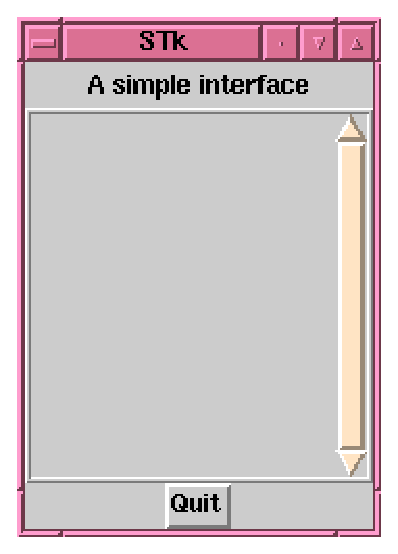
\epsfig{file=Basic-Fig-1.ps}}
\caption{A simple interface}
\label{fig-simple-interface}
\end{figure}
This interface is composed of three main components: 
\begin{enumerate}
\item a label which is situated at top
\item a frame which is itself constituted of two components: 
\begin{enumerate}
\item a listbox, and
\item a scrollbar
\end{enumerate}
\item a ``quit'' button
\end{enumerate}
Let's have look now to  the objects we'll have to create for this interface.
First we can create the top label and the quit button which are relatively
simple. This can be done with the following definitions:
\begin{quote}
\begin{verbatim}
(define lab  (make <Label>  :text "A simple interface"))
(define quit (make <Button> :text "Quit" :command '(exit)))
\end{verbatim}
\end{quote}
The {\tt :command} init-keyword permits to associate an action to the button
(this action will be triggered when the mouse button 1 will be released over
the {\tt quit} button.

The interface shown in Figure~\ref{fig-simple-interface} can be seen as a vertical alignment of
 three components (a label, a listbox with a scrollbar and a button). The
second component is itself an alignment of two object (a scrollbar and a
listbox). What is important to note here is that this alignment is an
horizontal one situated inside a vertical one. In this case, we have to place
the components of our horizontal alignment in a container which acts as a kind
of back box for further layout. The widget which permit to ``embody'' several
widgets is called a frame in the Tk toolkit. Consequently, the listbox and its
scrollbar can be defined by:
\begin{quote}
\begin{verbatim}
(define box  (make <Frame> :border-width 3 :relief "ridge"))
(define l    (make <Listbox>   :parent box))
(define s    (make <Scrollbar> :parent box :orientation "vertical"))
\end{verbatim}
\end{quote}
What is important to note is that the listbox and the scrollbar both tell that
their {\em parent} is the frame {\tt box}. This is this indication which
effectively embody them in the frame.


All the basic components of our interface have been created. What it
rests to do consists to place the graphic components we have just defined
onto screen. First we can map the listbox and its scrollbar in the {\tt
box} object with the {\em packer}\index{packer} geometry manager (see
page \pageref{pack-doc}):
\begin{quote}
\begin{verbatim}
(pack l :expand #t :fill "both" :side "left")
(pack s :expand #t :fill "y" :side "right")
\end{verbatim}
\end{quote}
Both calls to {\tt pack} permit to define the arrangement of the listbox
and the scrollbar into the frame. Here we claim that the scrollbar should
stay on the right side of the frame and that it must expand itself only in
the vertical direction if its containing frame (i.e. {\tt box}) is resized.
Concerning the listbox, it will stay on rigth and it will fill all the
space ({\tt :fill~"both"}) if {\tt box} size changes.

Now we can {\em pack} the three components of this simple interface to show
up them on screen; it can be easily done by:
\begin{quote}
\begin{verbatim}
(pack lab box quit)
\end{verbatim}
\end{quote}
The complete program for the building the previous interface is given in
Figure~\ref{simple:the_code}.

\begin{figure}
{\footnotesize
\begin{verbatim}
;;; Defining the components
(define lab  (make <Label>  :text "A simple interface"))
(define quit (make <Button> :text "Quit" :command '(exit)))
(define box  (make <Frame>  :border-width 3 :relief "ridge"))

;;; Zoom in the box
(define l    (make <Listbox>   :parent box))
(define s    (make <Scrollbar> :parent box :orientation "vertical"))

(pack l :expand #t :fill "both" :side "left")
(pack s :expand #t :fill "y" :side "right")

;;; Pack the components
(pack lab box quit)
\end{verbatim}
}
\caption{Complete code for the simple interface}
\label{simple:the_code}
\end{figure}

\subsubsection{Filling the listbox}

Filling the listbox can be done by calling the {\tt insert}
\index{listbox insert} method. This method permits to add elements in the
listbox. A way to fill the previous lisbox could be:
\begin{quote}
\begin{verbatim}
(insert l 0 "a" "b" "c")
\end{verbatim}
\end{quote}
This will insert 3 lines (containing {\tt "a"}, {\tt "b"} and {\tt "c"})
after the element whose index is 0. Inserting a {\tt "d"} between {\tt "a"}
and {\tt "b"} could be done by the following expression:
\begin{quote}
\begin{verbatim}
(insert l 1 "d")
\end{verbatim}
\end{quote}

Deleting elements of listbox necessitates a call to the {\tt delete}
method. For instance,
\begin{quote}
\begin{verbatim}
(delete l 1)
\end{verbatim}
\end{quote}
deletes the second element of the listbox (first element is at index 0), and
\begin{quote}
\begin{verbatim}
(delete l 0 2)
\end{verbatim}
\end{quote}
permits to delete the three remaining elements. 

{\tt Insert} and {\tt delete} are simple methods built upon Tk commands to
accesss listbox. Most of the time, this way of accessing a listbox is not
too convenient, and it is more easy to see the content of a listbox as its
value. Consequently, the {\tt stklos} {\tt <Listbox>} class defines a
virtual slot\cite{virtual slot} called {\tt value}\index{value} which
permits to read/fill the contents of a listbox as a {\stklos} slot.
For instance, the previous listbox can be filled with:
\begin{quote}
\begin{verbatim}
(set! (value l) '("a" "b" "c"))  ;; or (slot-set! l 'value '(...))
\end{verbatim}
\end{quote}
and the value of the second element of the listbox can be obtained by
\begin{quote}
\begin{verbatim}
(list-ref (value l) 1)
\end{verbatim}
\end{quote}

Of course, the value slot has an initialization keword associated to it,
and the filling of the listbox could have been done during the definition
of the listbox:
\begin{quote}
\begin{verbatim}
(define l (make <Listbox> :parent box 
                          :value  '("a" "b" "c")))
\end{verbatim}
\end{quote}

\subsubsection{Bringing the scrollbar to life}

For now, the lisbox and the scrollbar are disconnected (i.e. moving the
listbox, with {\tt <Shift-Button2>} doesn't move the scrollbar and clicking
the scrollbar does nothing). To make both widgets working accordingly, we have
to associate a command to each widget. First, we can associate a command to
the scrollbar, such as moving it with mouse button will move the listbox. This
can be done with:
\begin{quote}
\begin{verbatim}
(set! (command s) (format #f "y-view ~S " (address-of l)))
\end{verbatim}
\end{quote}
which associates the prefix of a Scheme command to invoke to change the view
in the listbox when the user manipulates the scrollbar. This command is
partial and will be completed effectively when the user will click the
scrollbar (see the <Scrollbar> class description on
page~\pageref{Scrollbar-class} for more details).

This is at  half way of what we have to do for cleanly associate the scrollbar
and the listbox. On the listbox side, we have to associate a command for its 
vertical movement:
\begin{quote}
\begin{verbatim}
(set! (y-scroll-command l) 
      (format #f "scrollbar-set! ~S " (address-of s)))
\end{verbatim}
\end{quote}
Here again, the command associated to the listbox is a partial since it will
be completed by Tk when needed.

As we will see in a next chapter, {\em composite widgets} will permit
to hide all this stuff, and we will be able to define a new class
which will embody a listbox and one (or two) scrollbar.

\subsection{Defining Menus}

\subsubsection{Menu-buttons and Menus}
Tk provides two widgets for building a menu: {\em menubuttons} and
{\em menus}. Those widgets are available through the {\tt
<Menu-button>} and {\tt <Menu>} classes. Instances of {\tt
<Menu-button>} class display a textual string (or a bitmap) and are
associated with an instance of the {\tt <Menu>} class.

\subsubsection{Creating a simple menu bar}

The most current task with menus concerns menu bars
building. {\stklos} provides the convenience function \Indextt{make-menubar}
to ease to the construction of menu bars. To illustrate how this
function work, we'll present the call we must write to produce the
menu bar of Figure~\ref{Menus}.
\begin{figure}
\centerline{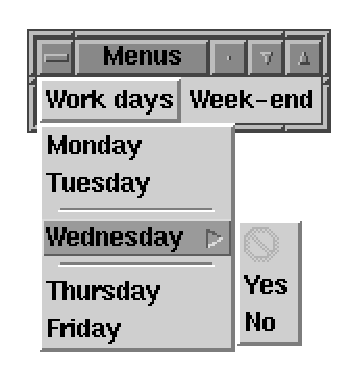
\epsfig{file=Fig2-2.eps}}
\caption{A simple menu}
\label{Menus}
\end{figure}
{\tt Make-menubar} is a function which takes a list of menu buttons
specifications. Each menu button specification is also a list.  First item
of this list is the specification of the menu button; the rest of this list
correspond to the specifaction of the menu items associated to this menu
button. To represent the menu bar of Figure\ref{Menus}, we have a
specification whih looks like:
\begin{quote}
\begin{alltt}
	((Description of {\it Work days} menu button
	     (Fisrt item of {\it Work days})
	     (Second item of {\it Work days}))
	 (Description of {\it Week end} menu button
	     (Fisrt item of {\it Week-end})
	     (Second item of {\it Week-end}))
	)
\end{alltt}
\end{quote}
The complete code for this menu bar is given in Figure\ref{Menus:code}.
Struture of menu buttons and menu items specifications is defined in
\ref{make-menubar}.
\begin{figure}
{\small
\begin{verbatim}
(define l `(("Work days" 
                 ("Monday"    ,(lambda () (format #t "Monday\n")))
                 ("Tuesday"   ,(lambda () (format #t "Tuesday\n")))
                 ("")
                 ("Wednesday"
                     ((command :bitmap error :state disabled)
                      ("Yes" ,(lambda () (format #t "Wednesday (Yes)\n")))
                      ("No"  ,(lambda () (format #t "Wednesday (No) \n")))))
                 ("")
                 ("Thursday"  ,(lambda () (format #t "Thursday\n")))
                 ("Friday"    ,(lambda () (format #t "Friday\n"))))
           ("Week-end"
                 ("Saturday"  ,(lambda () (format #t "Saturday\n")))
                 ("Sunday"    ,(lambda () (format #t "Sunday\n"))))))

(pack (make-menubar *top-root* l))
\end{verbatim}
}
\caption{Code of menu of Figure\ref{Menus}}
\label{Menus:code}
\end{figure}




\section{Simple widgets classes}
%%%%%%%%%%%%%%%%%%%%%%%%%%%%%%%%%%%%%%%%%%%%%%%%%%%%%%%%%%%%%%%%%%%%%%%%%%%%%%
% FRAME
%%%%%%%%%%%%%%%%%%%%%%%%%%%%%%%%%%%%%%%%%%%%%%%%%%%%%%%%%%%%%%%%%%%%%%%%%%%%%%

\subsection{The {\tt Frame} class}

A frame is a {\stklos} simple widget whose primary purpose is to act as a
spacer or container for complex window layouts. A frame object has several
Tk-virtual slots which are listed here:

\begin{ip}

\ITEM{background}
See section \ref{background}.

\ITEM{border-width}
See section \ref{border-width}.

\ITEM{cursor}
See section \ref{cursor}.

\ITEM{height}\label{height}
specifies the desired height for the window. This slot is only
used if the {\em geometry} slots is unspecified. If this pseudo-slot is less than 
or equal to zero (and {\em geometry} is not specified) then the window will 
not request any size at all.

\ITEM{geometry}\label{geometry}
specifies the desired geometry for the widget's window, in the
form {\em width}x{\em height}, where {\em width} is the desired
width of the window and {\em height} is the desired height.  The
units for {\em width} and {\em height} depend on the particular
widget.  For widgets displaying text the units are usually the
size of the characters in the font being displayed;  for other
widgets the units are usually pixels.

\ITEM{relief}
See section \ref{relief}.

\ITEM{width}
specifies the desired width for the window. This slot is only
used if the {\em geometry} slots is unspecified. If this pseudo-slot is less than 
or equal to zero (and {\em  geometry} is not specified) then the window will 
not request any size at all.
\end{ip}

\noindent
Furthermore, the {\em Frame} class admits a special initarg {\tt :class} which
permits to specify the new widget X11 resource class (if the {\tt :class} is
not passed as a parameter during the {\tt make-instance} of the frame, the
widget resource class will be "Frame"). The resource class of a widget can be
specified only at initialization. It can be queried by the {\tt class} reader
but cannot be changed.

Further example use a frame to group three labels in a single object. Here,
the two 
\begin{verbatim}
(setq f (make-instance 'Frame))
(setq l1 (make-instance 'Label :parent f :text " Label 1 " :relief :raised 
                               :map '(:position :left)))
(setq l2 (make-instance 'Label :parent f :text " Label 2 " :relief :raised 
                               :map '(:position :left)))
(setq l3 (make-instance 'Label :text " Label 3 " :relief :raised))
\end{verbatim}

%%%%%%%%%%%%%%%%%%%%%%%%%%%%%%%%%%%%%%%%%%%%%%%%%%%%%%%%%%%%%%%%%%%%%%%%%%%%%%
% LABEL
%%%%%%%%%%%%%%%%%%%%%%%%%%%%%%%%%%%%%%%%%%%%%%%%%%%%%%%%%%%%%%%%%%%%%%%%%%%%%%
\subsection{The label class}

The {\em Label} class defines widgets which are capable to display a textual
string or a bitmap. A label object has several pseudo-slots which are listed here:
\begin{ip}

\ITEM{anchor}\label{anchor}
specifies how the information in a widget (e.g. text or a bitmap) is to be
displayed in the widget. Must be one of the values {\em :n}, {\em :ne}, {\em
:e}, {\em :se}, {\em :s}, {\em :sw}, {\em :w}, {\em :nw}, or {\em `:center}.  For
example, {\em :nw} means display the information such that its top-left corner
is at the top-left corner of the widget.

\ITEM{background}
See section \ref{background}.

\ITEM{bitmap}\label{bitmap}
specifies a string containing the file name of the bitmap to display in the
widget. The exact way in which the bitmap is displayed may be affected by
other slots values such as {\em anchor} or {\em justify}.  Typically, if this
slot is non {\tt nil} is specified then it overrides other pseudo-slots that
specify a textual value to display in the widget; the {\em bitmap} slot may be
reset to an empty string to re-enable a text display.

\ITEM{border-width}
See section \ref{border-width}.

\ITEM{cursor}
See section \ref{cursor}.

\ITEM{font}\label{font}
specifies the font to use when drawing text inside the widget.

\ITEM{foreground}\label{foreground}
specifies the normal foreground color to use when displaying the widget.

\ITEM{height}
specifies a desired height for the label.  If a bitmap is being displayed in
the label then the value is in screen units; for text it is in lines of text.
If this pseudo-slot isn't specified, the label's desired height is computed from
the size of the bitmap or text being displayed in it.

\ITEM{pad-x}\label{pad-x}
specifies a non-negative value indicating how much extra space to request for
the widget in the X-direction. When computing how large a window it needs, the
widget will add this amount to the width it would normally need (as determined
by the width of the things displayed in the widget); if the geometry manager
can satisfy this request, the widget will end up with extra internal space to
the left and/or right of what it displays inside.

\ITEM{pad-y}\label{pad-y}
specifies a non-negative value indicating how much extra space to request for
the widget in the Y-direction. When computing how large a window it needs,
the widget will add this amount to the height it would normally need (as
determined by the height of the things displayed in the widget); if the
geometry manager can satisfy this request, the widget will end up with extra
internal space above and/or below what it displays inside.

\ITEM{relief}
See section \ref{relief}.

\ITEM{text}\label{text}
specifies a string to be displayed inside the widget.  The way in which
the string is displayed depends on the particular widget and may be
determined by other pseudo-slots, such as {\em anchor} or {\em justify}.

\ITEM{text-variable}\label{text-variable}
specifies the name of a variable. The value of the variable is a text
string to be displayed inside the widget; if the variable value changes
then the widget will automatically update itself to reflect the new value.
The way in which the string is displayed in the widget depends on the
particular widget and may be determined by other pseudo-slots, such as
{\em anchor} or {\em justify}. See below how to use this mechanism.

\ITEM{width}
Specifies a desired width for the label. If a bitmap is being displayed in
the label then the value is in screen units; for text it is in characters.  If
this pseudo-slot isn't specified, the label's desired width is computed from the
size of the bitmap or text being displayed in it.

\end{ip}

%%%%%%%%%%%%%%%%%%%%%%%%%%%%%%%%%%%%%%%%%%%%%%%%%%%%%%%%%%%%%%%%%%%%%%%%%%%%%%
% MESSAGE
%%%%%%%%%%%%%%%%%%%%%%%%%%%%%%%%%%%%%%%%%%%%%%%%%%%%%%%%%%%%%%%%%%%%%%%%%%%%%%
\section{The Message class}
The {\em Message} class defines widgets that display a textual string.  A {\em
message}widget has three special features. First, it breaks up its string into
lines in order to produce a given aspect ratio for the window.  The line
breaks are chosen at word boundaries wherever possible (if not even a single
word would fit on a line, then the word will be split across lines).  Newline
characters in the string will force line breaks; they can be used, for
example, to leave blank lines in the display.

The second feature of a message widget is justification.  The text may be
displayed left-justified, centered on a line-by-line basis, or right-justified.

The third feature of a message widget is that it handles control characters
and non-printing characters specially.  Tab characters are replaced with
enough blank space to line up on the next 8-character boundary.  Newlines
cause line breaks.  Other control characters (ASCII code less than hexadecimal
code 20) and characters not defined in the font are displayed as a
four-character sequence \\x{\it hh} where {\it hh} is the two-digit
hexadecimal number corresponding to the character.

\noindent
A message object has several pseudo-slots which are listed here:
\begin{ip}

\ITEM{anchor}
(see section \ref{anchor})

\ITEM{aspect}\label{aspect}
specifies a non-negative integer value indicating desired aspect ratio for the
text. The aspect ratio is specified as 100*width/height. 100 means the text
should be as wide as it is tall, 200 means the text should be twice as wide as
it is tall, 50 means the text should be twice as tall as it is wide, and so
on. Used to choose line length for text if {\em width} pseudo-slot isn't
specified.

\ITEM{background}
(see section \ref{background})

\ITEM{border-width}
(see section \ref{border-width})

\ITEM{cursor}
(see section \ref{cursor})

\ITEM{font}
(see section \ref{font})

\ITEM{justify}\label{justify}
specifies how to justify lines of text. Must be one of {\em :left}, {\em
:center}, or {\em :right}. Defaults to {\em left}. This pseudo-slot works
together with the {\em anchor}, {\em aspect}, {\em padX}, {\em padY}, and {\em
width} pseudo-slots to provide a variety of arrangements of the text within
the window.  The {\em aspect} and {\em width} pseudo-slots determine the
amount of screen space needed to display the text.  The {\em anchor}, {\em
padX}, and {\em padY} pseudo-slots determine where this rectangular area is
displayed within the widget's window, and the {\em justify} pseudo-slot determines
how each line is displayed within that rectangular region.  For example,
suppose {\em anchor} is {\em :e} and {\em justify} is {\em :left}, and that the
message window is much larger than needed for the text. The text will
displayed so that the left edges of all the lines line up and the right edge
of the longest line is {\em pad-x} from the right side of the window; the
entire text block will be centered in the vertical span of the window.
\ITEM{pad-x}
(see section \ref{pad-x})

\ITEM{pad-y}
(see section \ref{pad-y})

\ITEM{relief}
(see section \ref{relief})

\ITEM{text}
(see section \ref{text})

\ITEM{text-variable}
(see section \ref{text-variable})

\ITEM{width}\label{width}
specifies the length of lines in the window. If this pseudo-slot has a value
greater than zero then the {\em aspect} pseudo-slot is ignored and the {\em
width} pseudo-slot determines the line length.  If this pseudo-slot has a
value less than or equal to zero, then the {\em aspect} pseudo-slot determines
the line length.

\end {ip}

%%%%%%%%%%%%%%%%%%%%%%%%%%%%%%%%%%%%%%%%%%%%%%%%%%%%%%%%%%%%%%%%%%%%%%%%%%%%%%
% BUTTON
%%%%%%%%%%%%%%%%%%%%%%%%%%%%%%%%%%%%%%%%%%%%%%%%%%%%%%%%%%%%%%%%%%%%%%%%%%%%%%
\section{The Button class}

The {\em Button} class defines widgets that display a ``reactive'' textual
string or bitmap. It can display itself in either of three different ways,
according to the {\em state} pseudo-slot; it can be made to appear raised,
sunken, or flat; and it can be made to flash.  When a user invokes the button
(defaultly, by pressing mouse button 1 with the cursor over the button), then
the command specified in the {\em command} pseudo-slot is invoked. Several
methods are also defined for buttons. They are presented at end of chapter.

A button object has several pseudo-slots which are listed here:

\begin{ip}

\ITEM{active-background}\label{active-background}
specifies background color to use when drawing active elements.
An element (a widget or portion of a widget) is active if the
mouse cursor is positioned over the element and pressing a mouse button
will cause some action to occur.

\ITEM{active-foreground}\label{active-foreground}
specifies foreground color to use when drawing active elements.
See above for definition of active elements.

\ITEM{anchor}
(see section \ref{anchor})

\ITEM{background}
(see section \ref{background})

\ITEM{bitmap}
(see section \ref{bitmap})

\ITEM{border-width}
(see section \ref{border-width})

\ITEM{command}\label{command}
specifies a command to associate with the button. This command is typically
invoked when mouse button 1 is released over the button window.

\ITEM{cursor}
(see section \ref{cursor})

\ITEM{disabled-foreground}\label{disabled-foreground}
specifies foreground color to use when drawing a disabled element. If the
pseudo-slot is specified as an empty string (which is typically the case on
monochrome displays), disabled elements are drawn with the normal foreground
color but they are dimmed by drawing them with a stippled fill pattern.

\ITEM{font}
(see section \ref{font})

\ITEM{foreground}
(see section \ref{foreground})

\ITEM{height}
specifies a desired height for the button. If a bitmap is being displayed in
the button then the value is in screen units; for text it is in lines of text.
If this pseudo-slot isn't specified, the button's desired height is computed from
the size of the bitmap or text being displayed in it.

\ITEM{pad-x}
(see section \ref{pad-x})

\ITEM{pad-y}
(see section \ref{pad-y})

\ITEM{relief}
(see section \ref{relief})

\ITEM{state}
specifies one of three states for the button:  {\em :normal}, {\em :active},
or {\em `:disabled}.  In normal state the button is displayed using the
{\em foreground} and {\em background} pseudo-slots.  The active state is
typically used when the pointer is over the button.  In active state
the button is displayed using the {\em activeForeground} and
{\em activeBackground} pseudo-slots.  Disabled state means that the button
is insensitive:  it doesn't activate and doesn't respond to mouse
button presses.  In this state the {\em disabledForeground} and
{\em background} pseudo-slots determine how the button is displayed.

\ITEM{text}
(see section \ref{text})

\ITEM{text-variable}
(see section \ref{text-variable})

\ITEM{width}
Specifies a desired width for the button.  If a bitmap is being displayed in
the button then the value is in screen units;for text it is in characters.  If
this option isn't specified, the button's desired width is computed from the
size of the bitmap or text being displayed in it.

\end {ip}
\noindent
{\em Example}
The following example show a simple use of buttons. 
{\tt 
\begin{quote}
\begin{verbatim}
(setq b1 (make-instance 'Button :text "Yes" 
                                :command '(format t "You said Yes")))
(setq b2 (make-instance 'Button :text "No"
                                :command '(format t "You said No")))
(event-loop)
\end{verbatim}
\end{quote}}

%anchor
%background
%bitmap
%borderwidth
%cursor
%font
%foreground
%pad-x
%pad-y
%relief
%text
%text-variable

\section {Functions of this chapter}


%%%%%%%%%%%%%%%%%%%%%%%%%%%%%%%%%%%%%%%%%%%%%%%%%%%%%%%%%%%%%%%%%%%%%%%%%%%%%%
\chapter{Simple widget methods}
\section{pack}
\section{raise}
\section{lower}

%%%%%%%%%%%%%%%%%%%%%%%%%%%%%%%%%%%%%%%%%%%%%%%%%%%%%%%%%%%%%%%%%%%%%%%%%%%%%%
\chapter{The Canvas widget}

\section{The <Canvas> class}

\section{The <Canvas-item> class}
\subsection{<Rectangle> class}
\subsection{<Oval> class}

......\\
......\\
......
\section{Grouping canvas item objects}

\ldots
%%%%%%%%%%%%%%%%%%%%%%%%%%%%%%%%%%%%%%%%%%%%%%%%%%%%%%%%%%%%%%%%%%%%%%%%%%%%%%
\chapter{The Text widget}

\section{The <Text> class}
\section{The <Text-tag> class}
\section{The <Text-mark>}

%%%%%%%%%%%%%%%%%%%%%%%%%%%%%%%%%%%%%%%%%%%%%%%%%%%%%%%%%%%%%%%%%%%%%%%%%%%%%%

\chapter{Composite widgets}
\section{Standard composite widgets}

\subsection{Labeled Entry}
\subsection{Default button}
\subsection{Choice button}
\subsection{Paned window}
\subsection{Scrool Listbox}
\subsection{Scroll Text}
\subsection{Scroll Canvas}
\subsection{File box}

\section{Writing composite widgets}

%
% STklos + Tk  Documentation
%
%           Author: Erick Gallesio [eg@kaolin.unice.fr]
%    Creation date:  4-Nov-1992 15:37
% Last file update:  5-Jun-1995 14:04

\documentclass[10pt]{report}
\usepackage{a4wide}
\usepackage{alltt}
\usepackage[dvips]{epsfig}
\usepackage{fancyheadings}
\usepackage{fancybox}

\pagestyle{fancyplain}
\makeindex
\parindent0pt
\parskip2mm
\begin{document}

%
% Commands
% 

%%%% STklos
\newcommand{\stk}{{\sc STk}}
\newcommand{\stklos}{{\sc STklos}}
\newcommand{\Indextt}[1]{{\tt{#1}}\index{#1}}
\newcommand{\Index}[1]{{#1}\index{#1}}

%%%% schemetitle
%\newcommand{\schemetitle}[2]{\vbox{\vskip0.5cm\hrule\vskip10pt\noindent
%{\tt\LARGE{#1}\index{#1}}\hfill{\em{#2}}\vskip10pt\hrule}\penalty10000}

\newcommand{\schemetitle}[2]{%
\begin{center}
\vskip2mm
\Ovalbox{\parbox{0.95\textwidth}{%
\vskip1mm~~{\tt\LARGE{#1}\index{#1}}\hfill{\tt{#2}}~~\vskip1mm}}
\vskip2mm
\end{center}}


%%%% ITEM
\newcommand{\ITEM}[1]{\item[{\bf{#1}}]\index{#1}\item[]}

%
% Environments
%
%\newenvironment{schemedoc}[1]{\vskip3mm\noindent{\em #1}\samepage
%\begin{list} {} {\setlength {\rightmargin}{0cm}\setlength {\leftmargin}
%{1cm}\setlength {\topsep} {0cm}\setlength {\partopsep} {0cm}
%\setlength {\parskip} {0cm}\item}}{\end{list}}
\newenvironment{schemedoc}[1]{\vskip0mm\noindent{\em #1}
\begin{list} {} {\setlength {\rightmargin}{0cm}\setlength {\leftmargin}
{1cm}\setlength {\topsep} {0cm}\setlength {\partopsep} {0cm}
\setlength {\parskip} {0cm}\item}}{\end{list}}

%%%% ip
\newenvironment{ip}{\noindent
\begin{list} {} {\setlength {\rightmargin}{0cm}
\setlength {\leftmargin}{2cm}
\setlength {\topsep} {0cm}
\setlength {\labelsep} {0cm}
\setlength {\listparindent} {0cm}
\setlength {\partopsep} {0cm}
\setlength {\parskip} {0cm}
\item}}{\end{list}\vskip3mm}


%
% Title page
%
\thispagestyle{empty}
\begin{center}   
\ \\[3cm]
{\huge\bf Using ST{\large\bf{KLOS}} for graphic programming}\\[3mm]
{\large or}\\[4mm]
{\large\bf{``Programming the Tk toolit with an OO Scheme''}}\\[3cm]
{\large Erick Gallesio ({\tt eg\@unice\.fr})}\\
{\large\em any other volunteers are welcome}
\end{center}
\vskip10cm
\begin{flushright}
April 1995
\end{flushright}
%
% Table of content
%
\tableofcontents

\input{Chap1}
\input{Chap2}
%%%%%%%%%%%%%%%%%%%%%%%%%%%%%%%%%%%%%%%%%%%%%%%%%%%%%%%%%%%%%%%%%%%%%%%%%%%%%%
\chapter{Simple widget methods}
\section{pack}
\section{raise}
\section{lower}

%%%%%%%%%%%%%%%%%%%%%%%%%%%%%%%%%%%%%%%%%%%%%%%%%%%%%%%%%%%%%%%%%%%%%%%%%%%%%%
\chapter{The Canvas widget}

\section{The <Canvas> class}

\section{The <Canvas-item> class}
\subsection{<Rectangle> class}
\subsection{<Oval> class}

......\\
......\\
......
\section{Grouping canvas item objects}

\ldots
%%%%%%%%%%%%%%%%%%%%%%%%%%%%%%%%%%%%%%%%%%%%%%%%%%%%%%%%%%%%%%%%%%%%%%%%%%%%%%
\chapter{The Text widget}

\section{The <Text> class}
\section{The <Text-tag> class}
\section{The <Text-mark>}

%%%%%%%%%%%%%%%%%%%%%%%%%%%%%%%%%%%%%%%%%%%%%%%%%%%%%%%%%%%%%%%%%%%%%%%%%%%%%%

\chapter{Composite widgets}
\section{Standard composite widgets}

\subsection{Labeled Entry}
\subsection{Default button}
\subsection{Choice button}
\subsection{Paned window}
\subsection{Scrool Listbox}
\subsection{Scroll Text}
\subsection{Scroll Canvas}
\subsection{File box}

\section{Writing composite widgets}

\input{STklos+Tk.ind}
\end{document}



\end{document}



\end{document}



\end{document}


